\setcounter{section}{1}
\section{PHƯƠNG TRÌNH BẬC NHẤT HAI ẨN, HỆ HAI PHƯƠNG TRÌNH BẬC NHẤT HAI ẨN}
\subsection{Trọng tâm kiến thức}
\begin{tomtat}
\subsubsection{Phương trình bậc nhất hai ẩn}
\begin{boxdn}
	\begin{itemize}
	\item Phương trình bậc nhất hai ẩn $x$, $y$ là phương trình có dạng
	\[ax+by=c,\]
	trong đó $a$, $b$, $c$ là các số đã biết (gọi là hệ số), $a$ và $b$ không đồng thời bằng $0$.
	\item Nếu giá trị của vế trái tại $x=x_0$ và $y=y_0$ bằng vế phải thì cặp số $\left(x_0;y_0\right)$ được gọi là một nghiệm của phương trình.
	\\ Giải phương trình là tìm tất cả các nghiệm của phương trình đó.
	\end{itemize}
\end{boxdn}
\begin{note}
	\begin{enumerate}[\bf --]
	\item Mỗi nghiệm $\left(x_0;y_0\right)$ của phương trình $ax+by=c$ được biểu diễn bởi điểm có tọa độ $\left(x_0;y_0\right)$ trên mặt phẳng tọa độ $Oxy$.
	\item Phương trình bậc nhất hai ẩn $ax+by=c$ luôn luôn có vô số nghiệm. Tất cả các nghiệm của nó được biểu diễn bởi một đường thẳng.
	\end{enumerate}
\end{note}
\begin{nx}
	Trong mặt phẳng tọa độ, tập hợp các điểm có tọa độ $(x;y)$ thỏa mãn phương trình bậc nhất hai ẩn $ax+by=c$ là một đường thẳng. Đường thẳng đó gọi là \textcolor{red}{đường thẳng $ax+by=c$}.
\end{nx}
\subsubsection{Hệ hai phương trình bậc nhất hai ẩn}
\begin{boxdn}
	\begin{itemize}
	\item Hệ hai phương trình bậc nhất hai ẩn $x,y$ có dạng:
	$\text{(I)} \heva{&a x+b y=c &&(1) \\ &a' x+b' y=c' &&(2)}$\\
	Trong đó, $ a $, $ b $, $ c $, $ a' $, $ b' $, $ c' $ là các số đã biết (gọi là hệ số), $ a $ và $ b $ không đồng thời bằng $ 0 $, $a'$ và $b'$ không đồng thời bằng $ 0 $.
	\item Nếu $\left(x_0; y_0\right)$ là nghiệm chung của hai phương trình $(1)$, $(2)$ thì $\left(x_0 ;y_0\right)$ được gọi là một \textit{nghiệm} của hệ $ \text{(I)} $.\\
	\textit{Giải hệ phương trình} là tìm tất cả các nghiệm của hệ phương trình đó.
	\end{itemize}
\end{boxdn}
\immini{
	\begin{note}
	Cặp số $(x_0;y_0)$ là nghiệm của hệ phương trình $(I)$ có nghĩa là điểm $M(x_0;y_0)$ vừa thuộc đường thẳng $d_1: ax+by=c$, vừa thuộc đường thẳng $d_2: a'x+b'y=c'$. Vậy $M$ là giao điểm của hai đường thẳng $d_1$ và $d_2$.
	\end{note}	
	}{
	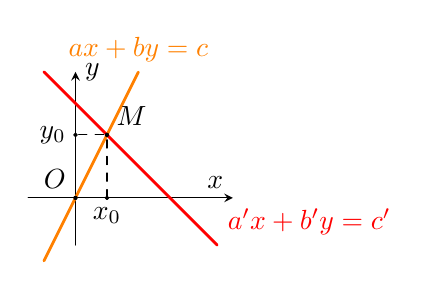
\begin{tikzpicture}[>=stealth,line join=round, line cap=round, scale=0.4]
	\draw[->] (-1.5,0)--(5,0) node[above left]{$x$};
	\draw[->] (0,-1.5)--(0,4) node[right]{$y$};
	\draw[samples=200,smooth,orange,line width=1] plot[domain=-1:2] 
	(\x,{2*\x}) node[above]{$ax+by=c$};
	\draw[samples=200,smooth,red,line width=1] plot[domain=-1:4.5] 
	(\x,{3-\x}) node[above right]{$a'x+b'y=c'$};
	\foreach \x in {1} \draw[fill] (\x,0) circle (1.5pt) 
	node[below]{$x_0$};
	\foreach \y in {2} \draw[fill] (0,\y) circle (1.5pt) 
	node[left]{$y_0$};
	\draw[dashed] (1,0)--(1,2)--(0,2);
	\fill (0,0) circle (2pt) node[above left]{$O$};
	\fill (1,2) circle (2pt) node[above right]{$M$};
	\end{tikzpicture}
}
\end{tomtat}
%%%%%%%%%%%%%%%%%%%
\subsection{Các dạng bài tập}
%=================
\begin{dang}{Nhận biết phương trình, nghiệm của phương trình bậc nhất 2 ẩn}
%	Thay $x = x_0, y = y_0$ vào phương trình $a x + b y = c$.
%	\begin{itemize}
%	\item Nếu $a x_0 + b y_0= c$ thì cặp số $\left(x_0; y_0\right)$ gọi là nghiệm của phương trình $a x + b y = c$.
%	\item Nếu $a x_0 + b y_0\ne c$ thì cặp số $\left(x_0; y_0\right)$ không là nghiệm của phương trình $a x + b y = c$.
%	\end{itemize}
\end{dang}
%%=====Ví dụ 1
\begin{vd}
	Trong các hệ thức $4x+3y=5$; $0x+y=-1$; $0x+0y=3$, hệ thức nào là phương trình bậc nhất hai ẩn? Hệ thức nào không phải là phương trình bậc nhất hai ẩn?
	\loigiai{
	Cả ba hệ thức đều có dạng $ax+by=c$. Nhưng chỉ có hai hệ thức $4x+3y=5$ và $0x+y=-1$ thỏa mãn điều kiện $a \ne 0$ hoặc $b \ne 0$ nên là phương trình bậc nhất hai ẩn.\\
	Hệ thức $0x+0y=3$ có $a=b=0$, không thỏa mãn điều kiện trên nên hệ thức đó không phải là phương trình bậc nhất hai ẩn.
	}
\end{vd}
%%=====Ví dụ 1
\begin{vd}
	Trong các phương trình sau, phương trình nào là bậc nhất hai ẩn $x$, $y$?
	\begin{listEX}[4]
	\item $2x-y=1$.
	\item $0x+3y=9$.
	\item $5x+0y=-2$.
	\item $3x^2-y=7$.
	\end{listEX}
	\loigiai{
	Phương trình ở các câu a, b, c là phương trình bậc nhất hai ẩn $x$, $y$. Phương trình ở câu d không phải là phương trình bậc nhất hai ẩn $x$, $y$
	}
\end{vd}
%%=====Ví dụ 1
\begin{vd}
	Trong các phương trình sau, phương trình nào là phương trình bậc nhất hai ẩn? Xác định các hệ số $a$, $b$, $c$ của phương trình bậc nhất hai ẩn đó.
	\begin{listEX}[4]
	\item $3x+5y=-3$.
	\item $0x-2y=5$.
	\item $-4x+0y=5$.
	\item $0x+0y=8$.
	\end{listEX}
	\loigiai{
	\begin{enumerate}
	\item $3x+5y=-3$ là phương trình bậc nhất hai ẩn với $a=3$, $b=5$ và $c=-3$.
	\item $0x-2y=5$ là phương trình bậc nhất hai ẩn với $a=0$, $b=-2$ và $c=7$.
	\item $-4x+0y=5$ là phương trình bậc nhất hai ẩn với $a=-4$, $b=0$ và $c=5$.
	\item $0x+0y=8$ không phải là phương trình bậc nhất hai ẩn vì $a=b=0$.
	\end{enumerate}
	}
\end{vd}
\begin{vd}
	Xác định hệ số $a$, $b$, $c$ của mỗi phương trình bậc nhất hai ẩn sau:
	\begin{listEX}[4]
	\item $x+5y=-4$.
	\item $\sqrt{3}x+y=0$.
	\item $0x-\dfrac{3}{2}y=6$.
	\item $2x+0y=-1{,}5$.
	\end{listEX}
	\loigiai{
	\begin{enumerate}
	\item $x+5y=-4$ là phương trình bậc nhất hai ẩn với $a=1$, $b=5$ và $c=-4$.
	\item $\sqrt{3}x+y=0$ là phương trình bậc nhất hai ẩn với $a=\sqrt{3}$, $b=1$ và $c=0$.
	\item $0x-\dfrac{3}{2}y=6$ là phương trình bậc nhất hai ẩn với $a=0$, $b=-\dfrac{3}{2}$ và $c=6$.
	\item $2x+0y=-1{,}5$ là phương trình bậc nhất hai ẩn với $a=2$, $b=0$ và $c=-1{,}5$.
	\end{enumerate}
	}
\end{vd}
\begin{vd}
	Hãy viết một phương trình bậc nhất hai ẩn và chỉ ra một nghiệm của nó.
	\loigiai{
	Phương trình bậc nhất hai ẩn $x-y=3$. Cặp số $(4;1)$ là một nghiệm của phương trình $x-y=3$.
	}
\end{vd}
%%=====Ví dụ 2
\begin{vd}
	Cho phương trình $3x-y=1$. Trong hai cặp số $(1;2)$ và $(1;-2)$, cặp số nào là nghiệm của phương trình đã cho?
	\loigiai{
	\begin{itemize}
	\item Cặp số $(1;2)$ là nghiệm của phương trình đã cho vì $3\cdot 1-2=1$.
	\item Cặp số $(1;-2)$ không phải là nghiệm của phương trình đã cho vì $3\cdot 1-(-2)=5\neq 1$.
	\end{itemize}
	}
\end{vd}
\begin{vd}
	Trong các cặp số sau, cặp số nào là nghiệm của phương trình $2x-3y=5$?
	\begin{listEX}[3]
	\item $(1;-1)$.
	\item $(0;5)$.
	\item $(-2;-3)$.
	\end{listEX}
	\loigiai{
	\begin{enumerate}
	\item Thay $x=1$; $y=-1$, ta có $2\cdot1-3\cdot(-1)=5$.\\
	Vậy $(1;-1)$ là một nghiệm của phương trình đã cho.
	\item Thay $x=0$; $y=5$, ta có $2\cdot0-3\cdot5=-15\ne5$.\\
	Vậy $(0;5)$ không là nghiệm của phương trình đã cho.
	\item Thay $x=-2$; $y=-3$, ta có $2\cdot(-2)-3\cdot(-3)=5$.\\
	Vậy $(-2;-3)$ là một nghiệm của phương trình đã cho.
	\end{enumerate}
	}
\end{vd}
\begin{vd}
	Cho phương trình $2x+y=4$. Chứng minh rằng các cặp số $(2;0), (0;4)$ là nghiệm của phương trình trên.
	\loigiai{
	Do $2\cdot 2+0=4$ là khẳng định đúng nên cặp số $(2;0)$ là nghiệm của phương trình trên. Tương tự, cặp số $(0;4)$ cũng là nghiệm của phương trình trên.
	}
\end{vd}
%%=====Ví dụ 1
\begin{vd}
	Trong các cặp số $(2;-1)$ và $(1;0)$, cặp số nào là nghiệm của phương trình $4x+3y=5$?
	\loigiai{
	Cặp số $(2;-1)$ là một nghiệm của phương trình $4x+3y=5$, vì $4 \cdot 2 + 3 \cdot (-1)=5 $.\\
	Cặp số $(1;0)$ không là nghiệm của phương trình $4x+3y=5$, vì $4 \cdot 1 +3 \cdot 0 \ne 5$.
	}
\end{vd}
\begin{vd}%[9D3B1]
	Xét xem cặp số $(2;-1)$ có là nghiệm của mỗi phương trình sau không?
	\begin{enumEX}{3}
	\item $2x + 3y = 1$;
	\item $2x - 3y = 1$;
	\item $\dfrac{3}{2}x + 4y = - 1$.
	\end{enumEX}
	\loigiai
	{
	\begin{enumerate}
	\item Thay $x = 2 , y = - 1$ vào phương trình $2x + 3y = 1$, ta được
	\[2\cdot2 + 3 \cdot( - 1) = 4 - 3 = 1.\]
	Vậy cặp số $(2;-1)$ là nghiệm của phương trình $2x + 3y = 1$.
	\item Thay $x = 2 , y = - 1$ vào phương trình $2x - 3y = 1$, ta được
	\[2\cdot2 - 3 \cdot( - 1) = 4 + 3 = 7\ne 1.\]
	Vậy cặp số $(2;-1)$ không là nghiệm của phương trình $2x - 3y = 1$.
	\item Thay $x = 2 , y = - 1$ vào phương trình $\dfrac{3}{2}x + 4y = - 1$, ta được
	\[\dfrac{3}{2}\cdot2 + 4 \cdot( - 1) = 3 - 4 = -1.\]
	Vậy cặp số $(2;-1)$ là nghiệm của phương trình $\dfrac{3}{2}x + 4y = - 1$.
	\end{enumerate}
	}
\end{vd}
\begin{vd}%[9D3B1]
	Kiểm tra xem các cặp số $(3;-1),\left(\sqrt{2};1-\sqrt{2}\right) ,(81;-80),(2;1)$. Cặp số nào là nghiệm của phương trình $x+y=1$.
	\loigiai{
	Ta lần lượt xét:
	\begin{itemize}
	\item Thay $(3;-1)$ vào phương trình, ta được $3+(-1)=1\Leftrightarrow 2=1$ (vô lý).\\
	Vậy cặp $(3;-1)$ không là nghiệm của phương trình.
	\item Thay $\left(\sqrt{2};1-\sqrt{2}\right) $ vào phương trình, ta được $\sqrt{2}+1-\sqrt{2}=1$ (đúng).\\
	Vậy cặp $\left(\sqrt{2};1-\sqrt{2}\right) $ là nghiệm của phương trình.
	\item Thay $(81;-80)$ vào phương trình, ta được $81-80=1$ (đúng).\\
	Vậy cặp $(81;-80)$ là nghiệm của phương trình.
	\item Thay (2;1) vào phương trình, ta được $2+1=1\Leftrightarrow 3=1$ (vô lý).\\
	Vậy cặp $(2;1)$ không là nghiệm của phương trình.
	\end{itemize}
	}
\end{vd}
\begin{vd}
	Cho phương trình $3x+2y=4$.\hfill(1)
	\begin{enumerate}
	\item Trong hai cặp số $(1;2)$ và $(2;-1)$, cặp số nào là nghiệm của phương trình (1).
	\item Tìm $y_0$ để cặp số $\left(4;y_0\right)$ là nghiệm của phương trình (1).
	\item Tìm thêm hai nghiệm của phương trình (1).
	\end{enumerate}
	\loigiai{
	\begin{enumerate}
	\item Cặp số $(1;2)$ không phải là nghiệm của phương trình (1) vì $3\cdot 1+2\cdot 2=7\neq 4$.\\
	Cặp số $(2;-1)$ là nghiệm của phương trình (1) vì $3\cdot 2+2\cdot (-1)=4$.
	\item Vì cặp số $\left(4;y_0\right)$ là nghiệm của phương trình (1) nên
	\allowdisplaybreaks
	\begin{eqnarray*}
	3\cdot 4+2\cdot y_0&=&4\\
	12+2y_0&=&4\\
	2y_0&=&-8\\
	y_0&=&-4.
	\end{eqnarray*}
	Vậy $y_0=-4$.
	\item Cặp số $(0;2)$ là nghiệm của phương trình (1) vì $3\cdot 0+2\cdot 2=4$.\\
	Cặp số $(-2;5)$ là nghiệm của phương trình (1) vì $3\cdot (-2)+2\cdot 5=4$.
	\end{enumerate}
	}
\end{vd}
%%=====Ví dụ 2
\begin{vd}
	Giả sử $(x;y)$ là nghiệm của phương trình bậc nhất hai ẩn $x+2y=5$.
	\begin{enumerate}
	\item Hoàn thành bảng sau đây:
	\begin{center}
	\begin{tabular}{|c|c|c|c|c|c|}
	\hline
	$x$&$-2$& $-1$&$0$&?&?\\
	\hline
	$y$&?&?&?&$1$&$2$\\
	\hline
	\end{tabular}
	\end{center}
	Từ đó suy ra $5$ nghiệm của phương trình đã cho.
	\item Tính $y$ theo $x$. Từ đó cho biết phương trình đã cho có bao nhiêu nghiệm
	\end{enumerate}
	\loigiai{
	\begin{enumerate}
	\item Ta có 
	\begin{center}
	\begin{tabular}{|c|c|c|c|c|c|}
	\hline
	$x$&$-2$& $-1$&$0$&$3$&$1$\\
	\hline
	$y$&$\tfrac{7}{2}$&$3$&$\tfrac{5}{2}$&$1$&$2$\\
	\hline
	\end{tabular}
	\end{center}
	Vậy $5$ nghiệm của phương trình đã cho là: $\left(-2; \dfrac{7}{2}\right)$, $(-1;3)$, $\left(0;\dfrac{5}{2} \right)$, $(3;1)$, $(1;2)$.
	\item Ta có $y=\dfrac{5-x}{2}$. Với mỗi giá trị $x$ tùy ý cho trước, ta luôn tìm được một giá trị $y$ tương ứng. Do đó phương trình đã cho có vô số nghiệm.\\
	\end{enumerate}
	}
\end{vd}
\begin{vd}
	Cô Hạnh có hai khoản đầu tư với lãi suất là $8\%$ và $10\%$ mỗi năm. Cô Hạnh thu được tiền lãi từ hai khoản đầu tư đó là 160 triệu đồng mỗi năm. Viết phương trình bậc nhất hai ẩn cho hai khoản đầu tư của cô Hạnh và chỉ ra ba nghiệm của phương trình đó.
	\loigiai
	{ Gọi $x$ (triệu đồng) là khoản đầu tư với lãi suất là $8\%$ mỗi năm ($x>0$). Khi đó, tiền lãi thu được mỗi năm từ khoản đầu tư này là \[8\%\cdot x=\dfrac{2x}{25}\ (\mbox{triệu đồng}).\]
	Gọi $y$ (triệu đồng) là khoản đầu tư với lãi suất là $10\%$ mỗi năm ($y>0$). Khi đó, tiền lãi thu được mỗi năm từ khoản đầu tư này là \[10\%\cdot y=\dfrac{y}{10}\ (\mbox{triệu đồng}).\]
	Ta có phương trình bậc nhất hai ẩn $x$, $y$ cho hai khoản đầu tư của cô Hạnh là 
	\[\dfrac{2x}{25}+\dfrac{y}{10}=160\ \mbox{hay }4x+5y=8\, 000.\]
	Ba nghiệm của phương trình trên là $(100; 1\, 520), (500;1\,200),(1\, 000;800)$.
	}
\end{vd}
\begin{vd}
	Hai bạn Dũng, Huy vào mua siêu thị mua vở và bút bi để ủng hộ các bạn học sinh vùng lũ lụt. Bạn Dũng mua 5 quyển vở và 3 chiếc bút bi với tổng số tiền phải trả là $39\, 000$ đồng. Bạn Huy mua 6 quyển vở và 2 chiếc bút bi với tổng số tiền phải trả là $42\, 000$ đồng. Giả sử giá của mỗi quyển vở là $x$ đồng $(x>0)$, giá của mỗi chiếc bút bi là $y$ đồng $(y>0)$.
	\begin{enumerate}
	\item Viết hai phương trình bậc nhất hai ẩn $x$, $y$ lần lượt biểu thị tổng số tiền phải trả của bạn Dũng, bạn Huy.
	\item Cặp số $(x;y)=(6\, 000;3\, 000)$ có phải là nghiệm của từng phương trình bậc nhất đó hay không? Vì sao?
	\end{enumerate}
	\loigiai{\begin{enumerate}
	\item Hai phương trình tương ứng là $5x+3y=39\, 000$ và $6x+2y=42\, 000$.
	\item Vì $x$, $y$ đồng thời thỏa mãn cả hai phương trình nói trên nên ta nói \\ cặp $(x;y)=(6\, 000;3\, 000)$ là nghiệm của hệ phương trình \[\heva{& 5x+3y=39\, 000 \\ & 6x+2y=42\, 000}.\]
	\end{enumerate}}
\end{vd}
%=================
%=================
\begin{dang}{Phương trình chứa tham số}
\end{dang}
\begin{vd}%[9D3B1]
	Nếu cặp số $(1;-2)$ là một nghiệm của phương trình $x - y - m = 0$ thì $m$ có giá trị là bao nhiêu?
	\loigiai
	{
	Vì cặp số $(1;-2)$ là một nghiệm của phương trình nên
	\[1 - ( - 2) - m = 0\Leftrightarrow m = 3.\]
	Vậy $m=3$.
	}
\end{vd}
\begin{vd}%[9D3B1]
	Để $(2m;-3)$ là một nghiệm của phương trình $3x +7y - 9 = 0$ thì $m$ có giá trị là bao nhiêu?
	\loigiai
	{
	Vì cặp số $(2m;-3)$ là một nghiệm của phương trình nên
	\[3\cdot2m + 7 \cdot( - 3) - 9 = 0\Leftrightarrow 6m - 30 = 0\Leftrightarrow m = 5.\]
	Vậy $m=5$.
	}
\end{vd}
\begin{vd}
	Tìm $m$ trong mỗi trường hợp sau
	\begin{enumEX}{1}
	\item $(1;2)$ là nghiệm của phương trình $mx+y-5=0$;
	\item Điểm $A(0;3)$ thuộc đường thẩng $4x+my-6=0$. 
	\end{enumEX}
	\loigiai{
	\begin{enumEX}{1}
	\item 
	Thay $x=1,\;y=2$ vào phương trình ta có $m \cdot 1 + 2 -5 = 0 \Leftrightarrow m=3.$
	\item 
	Thay $x=0,\;y=3$ vào đường thẳng, ta có $4 \cdot 0 + m \cdot 3 = 6 \Leftrightarrow m=2.$ 
	\end{enumEX}
	}
\end{vd}
\begin{vd}%[9D3G1]
	Chứng minh rằng khi $m$ thay đổi, các đường thẳng sau luôn đi qua một điểm cố định.
	\begin{listEX}[2]
	\item $3x+m(y-1)=2$;
	\item $mx+(m-2)y=m$.
	\end{listEX}
	\loigiai{
	\begin{enumerate}
	\item Giả sử $M(x_0;y_0)$ là điểm cố định mà đường thẳng luôn đi qua. Khi đó ta có\\
	$3x_0+m(y_0-1)-2=0\,\forall m\Leftrightarrow\heva{&3x_0-2=0\\&y_0-1=0}\Leftrightarrow\heva{&x_0=\dfrac{2}{3}\\&y_0=2}$.\\
	Vậy $M\left(\dfrac{2}{3};2\right) $ là điểm cố định mà đường thẳng luôn đi qua khi $m$ thay đổi.
	\item Giả sử $M(x_0;y_0)$ là điểm cố định mà đường thẳng luôn đi qua. Khi đó ta có\\
	$mx_0+(m-2)y_0=m\,\forall m\Leftrightarrow (x_0+y_0-1)m-2y_0=0\Leftrightarrow\heva{&x_0+y_0-1=0\\&-2y_0=0}\Leftrightarrow\heva{&x_0=1\\&y_0=0.}$\\
	Vậy $M(1;0)$ là điểm cố định mà đường thẳng luôn đi qua khi $m$ thay đổi.
	\end{enumerate}
	}
\end{vd}
%=================
\begin{dang}{Tìm nghiệm tổng quát và vẽ đường thẳng biểu diễn tập nghiệm phương trình}
	\begin{enumerate}[\itemKN]
	\item Tìm nghiệm tổng quát của phương trình $a x + b y = c$:
	\begin{itemize}
	\item Nếu $a\ne 0$ thì $x =\dfrac{c - b y}{a}$ và viết công thức nghiệm tổng quát là
	$\heva{&x =\dfrac{c - b y}{a} \\ &y\in \mathbb{R}.}$
	\item Nếu $b\ne 0$ thì $y =\dfrac{c - a x}{b}$ và viết công thức nghiệm tổng quát là
	$\heva{&x\in \mathbb{R} \\&y =\dfrac{c - a x}{b}.}$
	\end{itemize}
	\item Vẽ đường thẳng có phương trình $a x + b y = c$:
	\begin{itemize}
	\item Nếu $b\ne 0$ thì vẽ đường thẳng $y =\dfrac{1}{b}\cdot(c - a x)$.
	\item Nếu $b=0$ thì vẽ đường thẳng $x =\dfrac{c}{a}$ cùng phương với trục tung.
	\end{itemize}
	\end{enumerate}
\end{dang}
%-----------
\begin{vd}%[9D3K1]
	Tìm nghiệm tổng quát của mỗi phương trình sau và vẽ đường thẳng biểu diễn tập nghiệm của nó
	\begin{enumEX}{2}
	\item $2x + 3y = 6$;
	\item $3x + 0 \cdot y = 2$.
	\end{enumEX}
	\loigiai
	{
	\begin{enumerate}
	\item Ta có $2x + 3y = 6\Leftrightarrow y = - \dfrac{2}{3}x + 2$. Do đó, nghiệm tổng quát của phương trình là
	$\heva{&x\in \mathbb{R}\\ &y = - \dfrac{2}{3}x + 2 . }$\\
	Đồ thị:
	\begin{center}
	\begin{tikzpicture}[line join = round, line cap = round,>=stealth,thick,scale=0.8]
	\draw[samples=200,domain=-1:4,smooth] plot (\x, {-2/3*\x + 2}) node[rotate=-34,above] at (1.7,1){$y = -\dfrac{2}{3}x+2$};
	\draw[->,line width = 1pt] (-1,0)--(0,0) node[below right]{$O$}--(4.5,0) node[below]{$x$};
	\draw[->,line width = 1pt] (0,-1)--(0,3.5) node[right]{$y$};
	\foreach \x in {1,2,3} \draw[thin] (\x,1pt)--(\x,-1pt) node [below] {$\x$};
	\foreach \y in {1,2,3} \draw[thin] (1pt,\y)--(-1pt,\y) node [left] {$\y$};
	\end{tikzpicture}
	\end{center}
	\item Nghiệm tổng quát của phương trình là
	$\heva{&x = \dfrac{2}{3} \\ &y\in \mathbb{R}. }$\\
	Đồ thị:
	\begin{center}
	\begin{tikzpicture}[line join = round, line cap = round,>=stealth,thick,scale=0.6]
	\draw[->,line width = 1pt] (-1,0)--(0,0) node[below left]{$O$}--(4,0) node[below]{$x$};
	\draw[->,line width = 1pt] (0,-1)--(0,3.5) node[right]{$y$};
	\foreach \x in {3/2,3} \draw[thin] (\x,1pt)--(\x,-1pt);
	\foreach \y in {} \draw[thin] (1pt,\y)--(-1pt,\y) node [left] {$\y$};
	\draw (2,3.5)--(2,-1);
	\node at (2,0) [below left]{{\scriptsize $\dfrac{2}{3}$}};
	\node at (3,0) [below]{{\scriptsize $1$}};
	\node at (3,2) {{\scriptsize $x=\dfrac{2}{3}$}};
	\end{tikzpicture}
	\end{center}
	\end{enumerate}
	}
\end{vd}
\begin{vd}
	Viết nghiệm và biểu diễn hình học tất cả các nghiệm của mỗi phương trình bậc nhất hai ẩn sau:
	\begin{enumEX}{3}
	\item $x+2y=3$;
	\item $0x+y=-2$;
	\item $x+0y=3$.
	\end{enumEX}
	\loigiai{
	\begin{enumerate}
	\item 
	Xét phương trình $x+2y=3$. \quad $(1)$
	\immini{Ta viết $(1)$ dưới dạng $y=-0{,}5x +1{,}5$. Mỗi cặp số $(x;-0{,}5x +1{,}5)$ với $x \in \mathbb{R}$ tùy ý, là một nghiệm của $(1)$. Khi đó ta nói phương trình $(1)$ có nghiệm (tổng quát) là:
	\begin{center}
	$(x;-0,5x +1,5)$ với $x \in \mathbb{R}$ tùy ý.
	\end{center}
	Mỗi nghiệm này là tọa độ của một điểm thuộc đường thẳng $y=-0,5x +1,5$. Ta cũng gọi đường thẳng này là đường thẳng $d: x+2y=3$.
	}{
	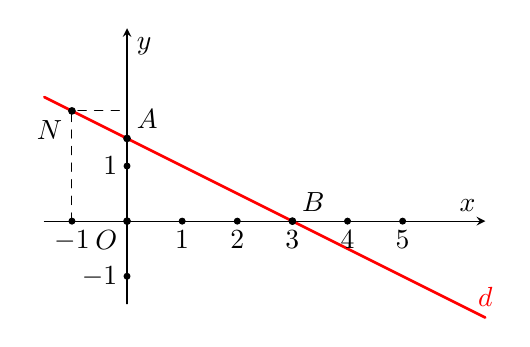
\begin{tikzpicture}[>=stealth,line join=round, line cap=round, scale=0.7]
	\draw[->] (-1.5,0)--(6.5,0) node[above left]{$x$};
	\draw[->] (0,-1.5)--(0,3.5) node[below right]{$y$};
	\draw[samples=200,smooth,red,line width=1] plot[domain=-1.5:6.5] 
	(\x,{(-0.5*\x)+1.5}) node[above]{$d$};
	\foreach \x in {-1,1,2,3,4,5} \draw[fill] (\x,0) circle (1.5pt) 
	node[below]{$\x$};
	\foreach \y in {-1,1} \draw[fill] (0,\y) circle (1.5pt) 
	node[left]{$\y$};
	\draw[dashed] (-1,0)--(-1,2)--(0,2);
	\fill (0,0) circle (2pt) node[below left]{$O$};
	\fill (-1,2) circle (2pt) node[below left]{$N$};
	\fill (0,1.5) circle (2pt) node[above right]{$A$};
	\fill (3,0) circle (2pt) node[above right]{$B$};
	\end{tikzpicture}
	}
	Để vẽ đường thẳng $d$, ta chỉ cần xác định hai điểm tùy ý của nó, chẳng hạn $A(0;1{,}5)$ và $B(3;0)$ rồi vẽ đường thẳng đi qua hai điểm đó.
	\item 
	Xét phương trình $0x+y=-2$. \quad $(2)$
	\immini{
	Ta viết gọn $(2)$ thành $y=-2$. Phương trình $(2)$ có nghiệm là $(x;-2)$ với $x \in \mathbb{R}$ tùy ý.\\
	Mỗi nghiệm này là tọa độ của một điểm thuộc đường thẳng song song với trục hoành và cắt trục tung tại điểm $(0;-2)$. Ta gọi đó là đường thẳng $y=-2$.}{
	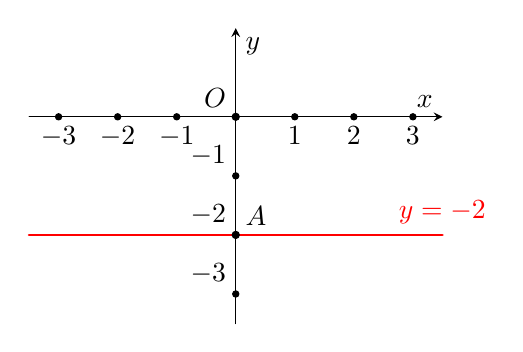
\begin{tikzpicture}[>=stealth,line join=round, line cap=round, scale=0.75]
	\draw[->] (-3.5,0)--(3.5,0) node[above left]{$x$};
	\draw[->] (0,-3.5)--(0,1.5) node[below right]{$y$};
	\draw[samples=200,smooth,red,line width=1] plot[domain=-3.5:3.5] 
	(\x,{-2}) node[above]{$y=-2$};
	\foreach \x in {-3,-2,-1,1,2,3} \draw[fill] (\x,0) circle (1.5pt) 
	node[below]{$\x$};
	\foreach \y in {-1,-2,-3} \draw[fill] (0,\y) circle (1.5pt) 
	node[above left]{$\y$};
	\fill (0,0) circle (2pt) node[above left]{$O$};
	\fill (0,-2) circle (2pt) node[above right]{$A$};
	\end{tikzpicture}
	}
	\item 
	Xét phương trình $x+0y=3$. \quad $(3)$
	\immini{
	Ta viết gọn $(3)$ thành $x=3$. Phương trình $(3)$ có nghiệm là $(3;y)$ với $x \in \mathbb{R}$ tùy ý.\\
	Mỗi nghiệm này là tọa độ của một điểm thuộc đường thẳng song song với trục tung và cắt trục hoành tại điểm $(3;0)$. Ta gọi đó là đường thẳng $x=3$ (H$1.1$c).}{
	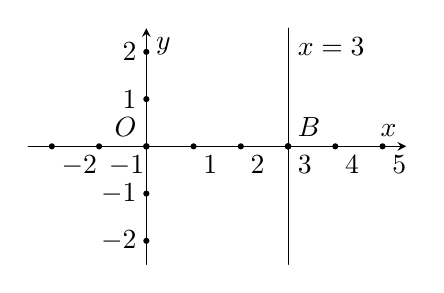
\begin{tikzpicture}[>=stealth,line join=round, line cap=round, scale=0.6]
	\draw[->] (-2.5,0)--(5.5,0) node[above left]{$x$};
	\draw[->] (0,-2.5)--(0,2.5) node[below right]{$y$};
	\draw[-] (3,-2.5)--(3,2.5) node[below right]{$x=3$};
	%	\draw[samples=200,smooth,red,line width=1] plot[domain=-2.5:2.5] 
	%	(\x,{-2}) node[above]{$x=3$};
	\foreach \x in {-2,-1,1,2,3,4,5} \draw[fill] (\x,0) circle (1.5pt) 
	node[below right]{$\x$};
	\foreach \y in {-2,-1,1,2} \draw[fill] (0,\y) circle (1.5pt) 
	node[left]{$\y$};
	\fill (0,0) circle (2pt) node[above left]{$O$};
	\fill (3,0) circle (2pt) node[above right]{$B$};
	\end{tikzpicture}
	}
	\end{enumerate}
	}
\end{vd}
\begin{vd}
	Viết nghiệm và biểu diễn hình học tất cả các nghiệm của mỗi phương trình bậc nhất hai ẩn sau:
	\begin{enumEX}{3}
	\item $2x-3y=5$;
	\item $0x+y=3$;
	\item $x+0y=-2$.
	\end{enumEX}
	\loigiai{
	\begin{enumerate}
	\item 
	Xét phương trình $2x-3y=5$. \quad $(1)$
	\immini{
	Ta viết $(1)$ dưới dạng $y=\dfrac{2}{3}x - \dfrac{5}{3}$. Mỗi cặp số $\left(x;\dfrac{2}{3}x - \dfrac{5}{3}\right)$ với $x \in \mathbb{R}$ tùy ý, là một nghiệm của $(1)$. Khi đó ta nói phương trình $(1)$ có nghiệm (tổng quát) là:
	\begin{center}
	$\left(x;\dfrac{2}{3}x - \dfrac{5}{3}\right)$ với $x \in \mathbb{R}$ tùy ý.
	\end{center}
	Mỗi nghiệm này là tọa độ của một điểm thuộc đường thẳng $y=\dfrac{2}{3}x - \dfrac{5}{3}$. Ta cũng gọi đường thẳng này là đường thẳng $d: 2x-3y=5$.
	}{
	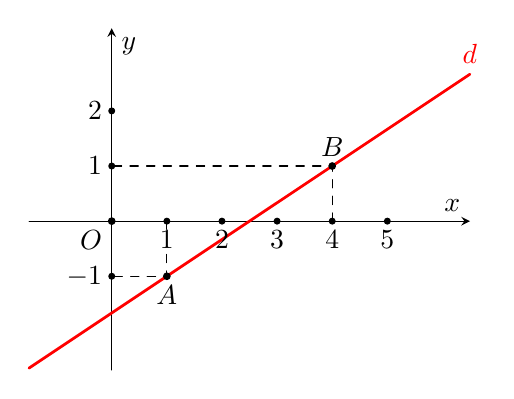
\begin{tikzpicture}[>=stealth,line join=round, line cap=round, scale=0.7]
	\draw[->] (-1.5,0)--(6.5,0) node[above left]{$x$};
	\draw[->] (0,-2.7)--(0,3.5) node[below right]{$y$};
	\draw[samples=200,smooth,red,line width=1] plot[domain=-1.5:6.5] 
	(\x,{(2/3*\x)-5/3}) node[above]{$d$};
	\foreach \x in {1,2,3,4,5} \draw[fill] (\x,0) circle (1.5pt) 
	node[below]{$\x$};
	\foreach \y in {-1,1,2} \draw[fill] (0,\y) circle (1.5pt) 
	node[left]{$\y$};
	\draw[dashed] (1,0)--(1,-1)--(0,-1);
	\draw[dashed] (4,0)--(4,1)--(0,1);
	\fill (0,0) circle (2pt) node[below left]{$O$};
	\fill (1,-1) circle (2pt) node[below]{$A$};
	\fill (4,1) circle (2pt) node[above]{$B$};
	\end{tikzpicture}
	}
	Để vẽ đường thẳng $d$, ta chỉ cần xác định hai điểm tùy ý của nó, chẳng hạn $A(1;-1)$ và $B(4;1)$ rồi vẽ đường thẳng đi qua hai điểm đó .
	\item 
	Xét phương trình $0x+y=3$. \quad $(2)$
	\immini{
	Ta viết gọn $(2)$ thành $y=3$. Phương trình $(2)$ có nghiệm là $(x;3)$ với $x \in \mathbb{R}$ tùy ý.\\
	Mỗi nghiệm này là tọa độ của một điểm thuộc đường thẳng song song với trục hoành và cắt trục tung tại điểm $(0;3)$. Ta gọi đó là đường thẳng $y=3$}{
	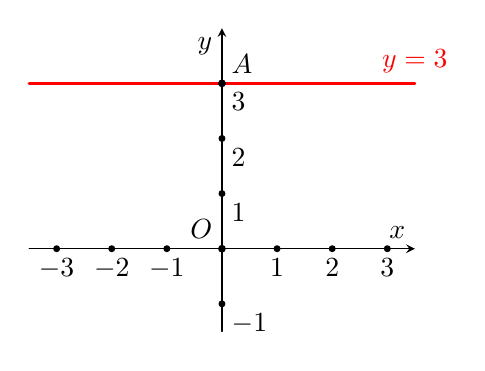
\begin{tikzpicture}[>=stealth,line join=round, line cap=round, scale=0.7]
	\draw[->] (-3.5,0)--(3.5,0) node[above left]{$x$};
	\draw[->] (0,-1.5)--(0,4) node[below left]{$y$};
	\draw[samples=200,smooth,red,line width=1] plot[domain=-3.5:3.5] 
	(\x,{3}) node[above]{$y=3$};
	\foreach \x in {-3,-2,-1,1,2,3} \draw[fill] (\x,0) circle (1.5pt) 
	node[below]{$\x$};
	\foreach \y in {-1,1,2,3} \draw[fill] (0,\y) circle (1.5pt) 
	node[below right]{$\y$};
	\fill (0,0) circle (2pt) node[above left]{$O$};
	\fill (0,3) circle (2pt) node[above right]{$A$};
	\end{tikzpicture}
	}
	\item 
	Xét phương trình $x+0y=-2$. \quad $(3)$
	\immini{
	Ta viết gọn $(3)$ thành $x=-2$. Phương trình $(3)$ có nghiệm là $(-2;y)$ với $x \in \mathbb{R}$ tùy ý.\\
	Mỗi nghiệm này là tọa độ của một điểm thuộc đường thẳng song song với trục tung và cắt trục hoành tại điểm $(-2;0)$. Ta gọi đó là đường thẳng $x=-2$.}{
	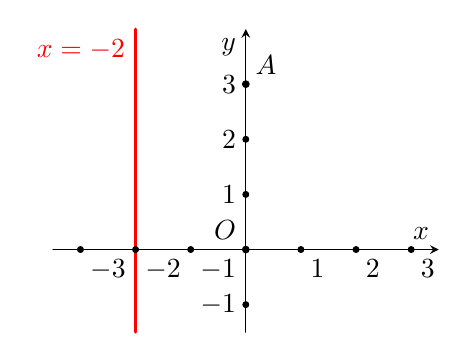
\begin{tikzpicture}[>=stealth,line join=round, line cap=round, scale=0.7]
	\draw[->] (-3.5,0)--(3.5,0) node[above left]{$x$};
	\draw[->] (0,-1.5)--(0,4) node[below left]{$y$};
	\draw[red,line width=1pt] (-2,-1.5)--(-2,4) node[below left]{$x=-2$};
	\foreach \x in {-3,-2,-1,1,2,3} \draw[fill] (\x,0) circle (1.5pt) 
	node[below right]{$\x$};
	\foreach \y in {-1,1,2,3} \draw[fill] (0,\y) circle (1.5pt) 
	node[left]{$\y$};
	\fill (0,0) circle (2pt) node[above left]{$O$};
	\fill (0,3) circle (2pt) node[above right]{$A$};
	\end{tikzpicture}
	}
	\end{enumerate}
	}
\end{vd}
\begin{vd}%[9D3K1]
	Cho phương trình $5x - 3y = 2$. \hfill $(1)$
	\begin{enumerate}
	\item Tìm công thức nghiệm tổng quát của phương trình $(1)$.
	\item Tìm nghiệm nguyên của phương trình.
	\end{enumerate}
	\loigiai
	{
	\begin{enumerate}
	\item Ta tính $y$ theo $x$
	\[5x - 3y = 2\Leftrightarrow 3y = 5x - 2\Leftrightarrow y =\dfrac{5x - 2}{3}.\]
	Phương trình có vô số nghiệm $\left(x ;\dfrac{5x - 2}{3}\right)$, với $x$ là một số thực tùy ý.
	\\
	Ta cũng có thể viết nghiệm của phương trình là $\heva{&x\in \mathbb{R} \\ &y =\dfrac{5x - 2}{3} .}$
	\item Ta có $y =\dfrac{5x - 2}{3}= 2x - 1 + \dfrac{1 - x}{3}$.\\
	Để $y\in\mathbb{Z}$ thì $\dfrac{1 - x}{3}\in\mathbb{Z}$.\\
	Đặt $\dfrac{1 - x}{3}= t~(t\in\mathbb{Z})\Rightarrow x = 1 - 3t$. Do đó
	\[y = 2(1 - 3t) - 1 + t\Leftrightarrow y = 1 - 5t.\]
	Vậy nghiệm tổng quát của phương trình là
	\[\heva{&x = 1 - 3t \\ &y = 1 - 5t},~t\in \mathbb{Z}.\]
	\end{enumerate}
	}
\end{vd}
\begin{vd}
	Cho phương trình $3x+2y=4$.\hfill(1)
	Hãy biểu diễn tất cả các nghiệm của phương trình (1) trên mặt phẳng tọa độ $Oxy$.
	\loigiai{
	\immini{
	Ta viết lại phương trình thành $y=\dfrac{-3}{2}x+2$. Từ đó, tất cả các nghiệm của phương trình $3x+2y=4$ được biểu diễn bởi đường thẳng $d$ đi qua hai điểm $(0;2)$ và $(-2;5)$.
	}{
	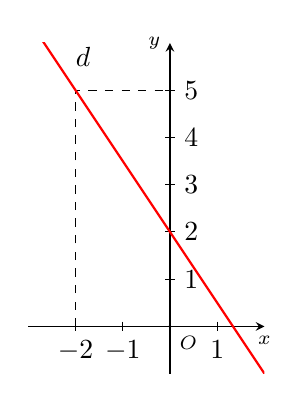
\begin{tikzpicture}[>=stealth,scale=0.6]
	\def\a{-1.5}
	\def\b{2}
	\draw[->] (-3,0) -- (2,0) node[below] {\scriptsize $x$};
	\draw[->] (0,-1) -- (0,6) node[left] {\scriptsize $y$};
	\fill (0,0) circle (1pt) node[below right]{\scriptsize $O$};
	\foreach \x in {-2,-1,1}{\draw (\x,0.1)--++(-90:0.2)node[below]{$\x$};}
	\foreach \y in {1,2,3,4,5}{\draw (-0.1,\y)--++(0:0.2)node[right]{$\y$};}
	\draw[dashed] (-2,0)|-(0,5);
	\clip (-3,-1)rectangle(2,6);
	\draw[thick,samples=150,smooth,domain=-3:2,red] plot(\x,{\a*\x+(\b)});
	\node[above right] at (-2.2,5.3){$d$};
	\end{tikzpicture}
	}
	}
\end{vd}
%%=====Ví dụ 3
\begin{vd}
	Biểu diễn tất cả các nghiệm của phương trình sau trên mặt phẳng tọa độ $Oxy$.
	\begin{listEX}[3]
	\item $-3x+y=2$.
	\item $0x+y=-2$.
	\item $2x+0y=3$.
	\end{listEX}
	\loigiai{
	\immini{
	\begin{enumerate}
	\item Viết lại phương trình thành $y=3x+2$. Từ đó, tất cả các nghiệm của phương trình đã cho được biểu diễn bởi đường thẳng $d:y=3x+2$.
	\end{enumerate}
	}{
	\begin{tikzpicture}[>=stealth,scale=0.8]
	\def\a{3}
	\def\b{2}
	\draw[->] (-2,0) -- (2,0) node[below] {\scriptsize $x$};
	\draw[->] (0,-1) -- (0,3) node[left] {\scriptsize $y$};
	\fill (0,0) circle (1pt) node[below right]{\scriptsize $O$};
	\foreach \x in {-1,1}{\draw (\x,-0.1)--++(90:0.2)node[above]{$\x$};}
	\foreach \y in {1,2}{\draw (-0.1,\y)--++(0:0.2)node[right]{$\y$};}
	\clip (-2,-1)rectangle(2,3);
	\draw[thick,samples=150,smooth,domain=-2:2,red] plot(\x,{\a*\x+(\b)})node[above]{$d$};
	\fill (-2/3,0) circle (1pt)node[below]{$\tfrac{2}{3}$};
	\node[below right] at (1/3,3){$d$};
	\end{tikzpicture}
	}
	\immini{
	\begin{enumerate}
	\item[b)] Viết lại phương trình thành $y=-2$. Từ đó, tất cả các nghiệm của phương trình đã cho được biểu diễn bởi đường thẳng $d$ vuông góc với $Oy$ tại điểm $M(0;-2)$.
	\end{enumerate}
	}{
	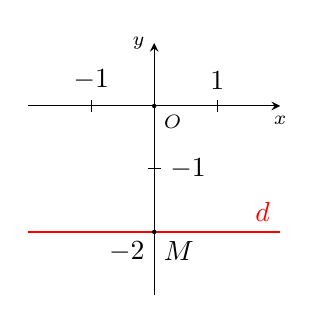
\begin{tikzpicture}[>=stealth,scale=0.8]
	\def\a{0}
	\def\b{-2}
	\draw[->] (-2,0) -- (2,0) node[below] {\scriptsize $x$};
	\draw[->] (0,-3) -- (0,1) node[left] {\scriptsize $y$};
	\fill (0,0) circle (1pt) node[below right]{\scriptsize $O$};
	\foreach \x in {-1,1}{\draw (\x,-0.1)--++(90:0.2)node[above]{$\x$};}
	\foreach \y in {-1}{\draw (-0.1,\y)--++(0:0.2)node[right]{$\y$};}
	\clip (-2,-3)rectangle(2,1);
	\draw[thick,samples=150,smooth,domain=-2:2,red] plot(\x,{\a*\x+(\b)})node[above left]{$d$};
	\fill (0,-2) circle (1pt)node[below left]{$-2$};
	\node[below right] at (0,-2){$M$};
	\end{tikzpicture}
	}
	\immini{
	\begin{enumerate}
	\item[c)] Viết lại phương trình thành $x=1{,}5$. Từ đó, tất cả các nghiệm của phương trình đã cho được biểu diễn bởi đường thẳng $d$ vuông góc với $Ox$ tại điểm $N(1{,}5;0)$.
	\end{enumerate}
	}{
	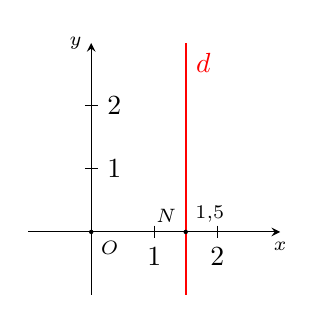
\begin{tikzpicture}[>=stealth,scale=0.8]
	\draw[->] (-1,0) -- (3,0) node[below] {\scriptsize $x$};
	\draw[->] (0,-1) -- (0,3) node[left] {\scriptsize $y$};
	\fill (0,0) circle (1pt) node[below right]{\scriptsize $O$};
	\foreach \x in {1,2}{\draw (\x,0.1)--++(-90:0.2)node[below]{$\x$};}
	\foreach \y in {1,2}{\draw (-0.1,\y)--++(0:0.2)node[right]{$\y$};}
	\draw[thick,samples=150,smooth,red] (1.5,-1)--(1.5,3)node[below right]{$d$};
	\fill (1.5,0) circle (1pt)node[above right]{\scriptsize $1{,}5$};
	\node[above left] at (1.5,0){\scriptsize $N$};
	\end{tikzpicture}
	}
	}
\end{vd}
\begin{vd}%[9D3K1]
	Tìm nghiệm nguyên của các phương trình:
	\begin{listEX}[3]
	\item $x-3y=4$.
	\item $3x+y=6$.
	\item $4x-5y=8$.
	\end{listEX}
	\loigiai{
	\begin{enumerate}
	\item Biến đổi phương trình về dạng $x=3y+4$.\\
	Nhận xét rằng, với mọi $y\in \mathbb{Z}$, ta luôn có $x=3y+4\in \mathbb{Z}$.\\
	Vậy phương trình có vô số nghiệm nguyên thỏa mãn $(3y+4;y)$ với $y\in \mathbb{Z}$.
	\item Biến đổi phương trình về dạng $y=-3x+6$.\\
	Nhận xét rằng, với mọi $x\in \mathbb{Z}$, ta luôn có $y=-3x+6\in \mathbb{Z}$.\\
	Vậy phương trình có vô số nghiệm nguyên thỏa mãn $(x;-3x+6)$ với $x\in \mathbb{Z}$.
	\item Biến đổi phương trình về dạng $4x=5y+8\Leftrightarrow x=y+2+\dfrac{y}{4}\quad (1)$.\\
	Đặt $k=\dfrac{y}{4},k\in \mathbb{Z}\Leftrightarrow y=4k,k\in \mathbb{Z}$.\\
	Thay $y=4k$ vào $(1)$ ta được $x=4k+2+k=5k+2\in \mathbb{Z},k\in \mathbb{Z}$.\\
	Vậy phương trình có vô số nghiệm nguyên thỏa mãn $(5k+2;4k)$ với $k\in \mathbb{Z}$.
	\end{enumerate}
	}
\end{vd}
%===================
\begin{dang}{Nhận biết hệ phương trình, nghiệm của hệ phương trình bậc nhất 2 ẩn}	
\end{dang}
%%=====Ví dụ 4
\begin{vd}
	Trong các hệ phương trình sau, hệ nào không phải là hệ hai phương trình bậc nhất hai ẩn, vì sao?
	\begin{enumEX}{3}
	\item $\heva{&2x=-6 \\&5x+4y=1;}$
	\item $\heva{&x+2y=-3 \\&0x+0y=1;}$
	\item $\heva{&3x-y=1 \\&x+y=3.}$
	\end{enumEX}
	\loigiai{
	Hệ phương trình b) không phải là hệ hai phương trình bậc nhất hai ẩn, vì phương trình thứ hai của hệ là $0x+0y=1$ không phải là phương trình bậc nhất hai ẩn.
	}
\end{vd}
\begin{vd}
	Trong những trường hợp sau, hãy chỉ ra các hệ hai phương trình bậc nhất hai ẩn:
	\begin{listEX}[4]
	\item $\heva{& 2x-3y=5 \\ & x+3y=-11;}$
	\item $\heva{& 2x-3y=5 \\ & 3x=-6;}$
	\item $\heva{& 9y=-27 \\ & x+3y=-11;}$
	\item $\heva{& x^2+y^2=121 \\ & x+3y=-11.}$
	\end{listEX}
	\loigiai{
	Hệ phương trình ở các câu $a$, $b$, $c$ là hệ hai phương trình bậc nhất hai ẩn. Trường hợp ở câu d không phải hệ phương trình bậc nhất hai ẩn.
	}
\end{vd}
\begin{vd}
	Trong các hệ phương trình sau, hệ phương trình nào là hệ hai phương trình bậc nhất hai ẩn?
	\begin{listEX}[3]
	\item $\heva{&x+3 y=3 \\&2 x+y=-4.}$
	\item $\heva{&0 x+0 y=-5 \\ &2 x+7 y=3.}$
	\item $\heva{&2 x+0 y=0 \\ &0 x-3 y=1.}$
	\end{listEX}
	\loigiai{
	\begin{enumerate}
	\item Hệ phương trình $\heva{&x+3 y=3 \\&2 x+y=-4}$ là hệ hai phương trình bậc nhất hai ẩn với $a=1$, $b=3,c=3$ và $a'=2$, $b'=1$, $c'=-4$.
	\item Hệ phương trình $\heva{&0 x+0 y=-5 \\&2 x+7 y=3}$ không phải là hệ hai phương trình bậc nhất hai ẩn vì $a=b=0$.
	\item Hệ phương trình $\heva{&2 x+0 y=0 \\&0 x-3 y=1}$ là hệ hai phương trình bậc nhất hai ẩn với $a=2$, $b=0$, $c=0$ và $a'=0$, $b'=-3$, $c'=1$.
	\end{enumerate}
	}
\end{vd}
\begin{vd}
	Trong các hệ phương trình sau, hệ phương trình nào là hệ hai phương trình bậc nhất hai ẩn?
	\begin{listEX}[3]
	\item $\heva{&x+3 y=0 \\ &4 x-3 y=-4.}$
	\item $\heva{&\sqrt{3} x+0 y=-5 \\&0 x+\frac{4}{5} y=3.}$
	\item $\heva{&7 x+2 y=-5 \\ &0 x+0 y=9.}$
	\end{listEX}
	\loigiai{
	\begin{listEX}
	\item Hệ phương trình $\heva{&x+3 y=0 \\ &4 x-3 y=-4}$ là hệ hai phương trình bậc nhất hai ẩn vì $ a=1 $, $ b=3 $, $ c=0 $ và $ a'=4 $, $ b'=-3 $, $ c'=-4 $.
	\item Hệ phương trình $\heva{&\sqrt{3} x+0 y=-5 \\&0 x+\frac{4}{5} y=3}$ là hệ hai phương trình bậc nhất hai ẩn vì $ a=\sqrt{3} $, $ b=0 $, $ c=-5 $ và $ a'=0 $, $ b'=\dfrac{4}{5} $, $ c'=3 $.
	\item Hệ phương trìn $\heva{&7 x+2 y=-5 \\ &0 x+0 y=9}$ không phải là hệ hai phương trình bậc nhất hai ẩn vì $ a'=b'=0 $.
	\end{listEX}
	}
\end{vd}
\begin{vd}
	Cho hệ phương trình $\heva{&x+5 y=10 \\&2 x-y=-13}$. Trong hai cặp số $(0 ; 2)$ và $(-5 ; 3)$, cặp số nào là nghiệm của hệ phương trình đã cho?
	\loigiai{
	Cặp số $(5 ;-3)$ là nghiệm của hệ phương trình vì $\heva{&-5+5\cdot 3=10 \\ &2\cdot(-5)-3=-13.}$\\
	Cặp số $(0;2)$ không là nghiệm của hệ phương trình vì $\heva{& 0+2 \cdot 5=10 \\& 2 \cdot 0-2=-2\,(\neq-13).}$
	}
\end{vd}
\begin{vd}
	Cho hệ phương trình $\heva{&2 x+3 y=7 \\&x-3 y=-1}$. Trong hai cặp số $(2 ; 1)$ và $(-1 ; 3)$, cặp số nào là nghiệm của hệ phương trình đã cho?
	\loigiai{
	Cặp số $(2 ; 1)$ là nghiệm của hệ phương trình vì $\heva{2\cdot 2+3\cdot 1=7 \\ 2-3\cdot 1=-1.}$\\
	Cặp số $(-1 ; 3)$ không là nghiệm của hệ phương trình vì $\heva{&2 \cdot(-1)+3 \cdot 3=7 \\& -1-3 \cdot 3=-10\,(\neq-1).}$
	}
\end{vd}
\begin{vd}
	Cho hệ phương trình $\heva{& 2x-3y=5 \\ & x+3y=-11.}$ \\ Trong các cặp số sau, cặp số nào là nghiệm của hệ phương trình đã cho?
	\begin{listEX}[2]
	\item $(-2;-3)$.
	\item $(1;-1)$.
	\end{listEX}
	\loigiai{
	\begin{enumerate}
	\item Thay giá trị $x=-2,y=-3$ vào mỗi phương trình trong hệ ta có $2\cdot(-2)-3\cdot(-3)=5$, $-2+3\cdot(-3)=-11$.\\
	Suy ra cặp số $(-2;-3)$ là nghiệm của từng phương trình trong hệ.\\
	Do đó cặp số $(-2;-3)$ là nghiệm của hệ phương trình đã cho.
	\item Thay giá trị $x=1,y=-1$ vào mỗi phương trình trong hệ ta có $2\cdot1-3\cdot(-1)=5$, $1+3\cdot(-1)=-2\ne-11$.\\
	Suy ra cặp số $(1;-1)$ không là nghiệm của phương trình thứ hai trong hệ.\\
	Do đó cặp số $(1;-1)$ không là nghiệm của hệ phương trình đã cho.
	\end{enumerate}
	}
\end{vd}
%%=====Ví dụ 5
\begin{vd}
	Cho hệ phương trình $\heva{& 2x-5y=-2 \\ & x+y=6.}$.
	Kiểm tra xem cặp số nào sau đây là nghiệm của hệ phương trình đã cho
	\begin{listEX}[2]
	\item $(3;3)$.
	\item $(4;2)$.
	\end{listEX}
	\loigiai{
	\begin{enumerate}
	\item Thay giá trị $x=3,y=3$ vào mỗi phương trình trong hệ ta có $$2\cdot3-5\cdot3=-9\ne 2.$$
	Suy ra cặp số $(3;3)$ không là nghiệm hệ phương trình đã cho.
	\item Thay giá trị $x=4,y=2$ vào mỗi phương trình trong hệ ta có $$2\cdot4-5\cdot2=-2, 4+2=6.$$
	Suy ra cặp số $(4;2)$ là nghiệm của phương trình đã cho.
	\end{enumerate}
	}
\end{vd}
\begin{vd}
	Trong hai cặp số $(0;-2)$ và $(2;-1)$, cặp số nào là nghiệm của hệ phương trình $\heva{&x-2y=4 \\&4x+3y=5}?$
	\loigiai{
	\begin{itemize}
	\item Ta thấy khi $x=0$ và $y=-2$ thì:\\
	$4x+3y=4 \cdot 0 +3 \cdot (-2)=-6 \ne 5$ nên $(0;-2)$ không là nghiệm của phương trình thứ hai. Vậy $(0;-2)$ không là nghiệm của hệ phương trình đã cho.
	\item Ta thấy khi $x=2$ và $y=-1$ thì:\\
	$x-2y=2-2 \cdot (-1)=4$ nên $(2;-1)$ là nghiệm của phương trình thứ nhất;\\
	$4x+3y=4 \cdot 2 +3 \cdot (-1)=5$ nên $(2;-1)$ là nghiệm của phương trình thứ hai.\\
	Vậy $(2;-1)$ là nghiệm chung của hai phương trình, nghĩa là $(2;-1)$ là một nghiệm của hệ phương trình đã cho.
	\end{itemize}
	}
\end{vd}
%%=====Ví dụ 5
\begin{vd}
	Giải thích tại sao cặp số $(1;2)$ là một nghiệm của hệ phương trình $\heva{&2x-y=0 \\&x+y=3.}$
	\loigiai{
	Ta thấy khi $x=1$ và $y=2$ thì:
	\begin{itemize}
	\item $2x-y=2 \cdot 1 -2=0$ nên $(1;2)$ là nghiệm của phương trình thứ nhất;
	\item $x+y=1+2=3$ nên $(1;2)$ là nghiệm của phương trình thứ hai.
	\end{itemize}
	Vậy $(1;2)$ là nghiệm chung của hai phương trình, nghĩa là $(1;2)$ là một nghiệm của hệ phương trình đã cho.
	}
\end{vd}
\begin{vd}
	Xét bài toán cổ sau:
	\begin{center}
	\textit{Quýt, cam mười bảy quả tươi\\
	Đem chia cho một trăm người cùng vui.\\
	Chia ba mỗi quả quýt rồi,\\
	Còn cam, mỗi quả chia mười vừa xinh.\\
	Trăm người, trăm miếng ngọt lành.\\
	Quýt, cam mỗi loại tính rành là bao?}
	\end{center}
	Gọi $x$ là số cam, $y$ là số quýt cần tính $(x, y \in \mathbb{N}^*)$, ta có hệ phương trình bậc nhất hai ẩn sau: 
	$$\heva{&x+y=17 \\&10x+3y=100}$$
	Trong hai cặp số $(10;7)$ và $(7;10)$, cặp số nào là nghiệm của hệ phương trình trên? Từ đó cho biết một phương án về số cam và số quýt thỏa mãn yêu cầu của bài toán cổ.
	\loigiai{
	\begin{itemize}
	\item 	Ta thấy khi $x=10$ và $y=7$ thì:\\
	$10x+3y=10 \cdot 10 +3 \cdot 7=121 \ne 100$ nên $(10;7)$ không là nghiệm của phương trình thứ hai. Vậy $(10; 7)$ không là nghiệm của hệ phương trình đã cho.
	\item Ta thấy khi $x=7$ và $y=10$ thì:\\
	$x+y=7+10=17$ nên $(7;10)$ là nghiệm của phương trình thứ nhất;\\
	$10x+3y=10 \cdot 7 +3 \cdot 10=100$ nên $(7;10)$ là nghiệm của phương trình thứ hai.
	\end{itemize}
	Do đó $(7;10)$ là nghiệm chung của hai phương trình, nghĩa là $(7;10)$ là một nghiệm của hệ phương trình đã cho.\\
	Vậy nên chia 7 quả cam mỗi quả thành 10 phần bằng nhau và chia 10 quả quýt mỗi quả thành 3 phần bằng nhau thì thỏa mãn yêu cầu của bài toán.
	}
\end{vd}
\begin{vd}
	Đối với bài toán:
	\begin{center}
	\textit{\lq\lq Một đàn em nhỏ đứng bên sông\\
	To nhỏ bàn nhau chuyện chia hồng\\
	Mỗi người năm trái thừa năm trái\\
	Mỗi người sáu trái một người không\\
	Hỡi người bạn trẻ đang dừng bước\\
	Có mấy em thơ, mấy trái hồng?\\
	Làm thế nào đế tính được số em nhỏ (em thơ) và số trái hồng?\rq\rq}
	\end{center}
	nếu gọi $x$ là số em nhỏ, $ y $ là số quả hồng thì ta nhận được hệ hai phương trình bậc nhất hai ẩn nào?
	\loigiai{
	Gọi $x$ là số em nhỏ, $ y $ là số quả hồng.\\
	Vì mỗi người $ 5 $ quả thì thừa $ 5 $ quả nên ta có: $ 5x+5 =y$. \hfill(1)\\
	Vì nỗi người $ 6 $ quả thì một người không có nên ta có: $ (x-1)\cdot 6 =y $. \hfill(2)\\
	Từ (1), (2) ta được hệ phương trình sau:
	\[\heva{&5x+5 =y\\&(x-1)\cdot 6 =y}\ \text{hay}\ \heva{&5x-y=5\\&6x-y=6.} \]
	}
\end{vd}
%===================
\begin{dang}{Đoán nhận số nghiệm của hệ phương trình}
	Cho hệ phương trình 
	$(I)~\heva{& ax+by=c &(d) \\ & a'x+b'y=c' &(d')}$
	\begin{itemize}
	\item Dựa vào hệ số góc và tung độ góc để biết số nghiệm của hệ, với $a'b'c'\ne 0$.
	\item Nếu $(d)$ cắt $(d')$ thì hệ $(I)$ có nghiệm duy nhất
	$\left( \dfrac{a}{a'}\ne \dfrac{b}{b'}\right)$.
	\item Nếu $(d)\parallel (d')$ thì hệ $(I)$ vô nghiệm
	$\left( \dfrac{a}{a'}=\dfrac{b}{b'}\ne \dfrac{c}{c'}\right)$.
	\item Nếu $(d)$ trùng với $(d')$ thì hệ $(I)$ có vô số nghiệm
	$\left(\dfrac{a}{a'}=\dfrac{b}{b'}= \dfrac{c}{c'}\right)$.
	\end{itemize}
\end{dang}
\begin{vd}%[9D3K1]
	Không cần vẽ hình, hãy cho biết số nghiệm của mỗi hệ phương trình sau đây và giải thích vì sao?
	\begin{enumEX}{3}
	\item $\heva{&y=2x-1 \\ &y=-x+1 }$;
	\item $\heva{&3x+2y=5 \\ &x-2y=2 }$;
	\item $\heva{&x+y=2 \\ &3x+3y=6 }$.
	\end{enumEX}
	\loigiai
	{
	\begin{enumerate}
	\item Vì $a\ne a'~(2\ne -1)$ nên hai đường thẳng đã cho cắt nhau.\\
	Vậy hệ có nghiệm duy nhất.
	\item Ta có 
	\[\heva{&3x+2y=5 \\ &x-2y=2 }\Leftrightarrow \heva{&y = - \dfrac{3}{2}x + \dfrac{5}{2}\\ &y =\dfrac{1}{2}x - 1.}\]
	Vì $a\ne a'~\left(-\dfrac{3}{2}\ne \dfrac{1}{2}\right)$ nên hai đường thẳng đã cho cắt nhau.\\
	Vậy hệ có nghiệm duy nhất.
	\item Ta có 
	\[\heva{&x+y=2 \\ &3x+3y=6 }\Leftrightarrow \heva{&y = - x + 2\\ &y = - x + 2.}\]
	Vì $a= a'~\left(=-1\right)$ và $c= c'~\left(=2\right)$ nên hai đường thẳng đã cho trùng nhau.\\
	Vậy hệ có vô số nghiệm.
	\end{enumerate}
	}
\end{vd}
\begin{vd}
	Không vẽ đồ thị, hãy đoán nhận số nghiệm các hệ phương trình sau
	\begin{enumEX}{3} 
	\item $\heva{&2x+y=1\\&x-y=1;}$
	\item $\heva{&x-y=2\\&-2x+2y=3;}$
	\item $\heva{&2x=3y \\ &x+5y=-4.}$
	\end{enumEX}
	\loigiai{
	\begin{enumEX}{1} 
	\item Ta có $$\heva{&2x+y=1\\&x-y=1}\Leftrightarrow \heva{&y=-2x+1\\&y=x-1.}$$
	Vì $a\ne a'~\left(-2\ne 1\right)$ nên hai đường thẳng đã cho cắt nhau.\\
	Vậy hệ có nghiệm duy nhất.
	\item Ta có $$\heva{&x-y=2\\&-2x+2y=3}\Leftrightarrow \heva{&y=x-2\\&y=x+\dfrac{3}{2}.}$$
	Vì $a= a'$ và $b\ne b'~\left(1=1; -2\ne \dfrac{3}{2}\right)$ nên hai đường thẳng đã cho song song.\\
	Vậy hệ vô nghiệm.
	\item Ta có 
	\[\heva{&2x=3y \\ &x+5y=-4 }\Leftrightarrow \heva{&y =\dfrac{2}{3}x\\ &y = - \dfrac{x}{5} - \dfrac{4}{5}.}\]
	Vì $a\ne a'~\left(\dfrac{2}{3}\ne -\dfrac{1}{5}\right)$ nên hai đường thẳng đã cho cắt nhau.\\
	Vậy hệ có nghiệm duy nhất.
	\end{enumEX}
	}
\end{vd}
%%%%%%%%%%%%%%%%%%%
\subsection{Bài tập vận dụng}
\begin{bt}
	Phương trình nào sau đây là phương trình bậc nhất hai ẩn, vì sao?
	\begin{enumEX}{4}
	\item $5x-8y=0$;
	\item $4x+0y=-2$;
	\item $0x+0y=1$;
	\item $0x-3y=9$.
	\end{enumEX}
	\loigiai{
	Các phương trình $5x-8y=0$, $4x+0y=-2$ và $0x-3y=9$ thỏa mãn điều kiện $a \ne 0$ hoặc $b \ne 0$ nên là phương trình bậc nhất hai ẩn.
	}
\end{bt}
\begin{bt}
	Trong các phương trình sau, phương trình nào là phương trình bậc nhất hai ẩn? Xác định các hệ số $ a $, $ b $, $ c $ của mỗi phương trình bậc nhất hai ẩn đó.
	\begin{listEX}[4]
	\item $2 x+5 y=-7$.
	\item $0 x-0 y=5$.
	\item $0 x-\dfrac{5}{4} y=3$.
	\item $0{,}2 x+0 y=-1{,}5$.
	\end{listEX}
	\loigiai{
	\begin{listEX}
	\item $2 x+5 y=-7$ là phương trình bậc nhất hai ẩn với $ a=2 $, $ b=5 $, $ c=-7 $.
	\item $0 x-0 y=5$ không phải là phương trình bậc nhất hai ẩn vì $ a=b=0 $.
	\item $0 x-\dfrac{5}{4} y=3$ là phương trình bậc nhất hai ẩn với $ a=0 $, $ b=-\dfrac{5}{4} $, $ c=3 $.
	\item $0{,}2 x+0 y=-1{,}5$ là phương trình bậc nhất hai ẩn vì $ a=0{,}2$, $b=0 $, $ c=-1{,}5 $.
	\end{listEX}
	}
\end{bt}
%%=====Bài 1
\begin{bt}
	Trong các cặp số $\left(8;1\right),\, \left(-3;6\right),\,\left(4;-1\right),\,\left(0;2\right)$, cho biết cặp số nào là nghiệm của mỗi phương trình sau:
	\begin{listEX}[2]
	\item $x-2y=6$;
	\item $x+y=3$.
	\end{listEX}
	\loigiai{
	\begin{enumerate}
	\item Thay cặp số $\left(x_0;y_0\right)$ vào phương trình $x-2y=6 \quad (1)$.
	\begin{itemize}
	\item Với $\left(8;1\right) \Rightarrow \heva{&x=8\\ &y=1}$ thay vào $(1)$, ta có $8-2\cdot 1=6$\\ 
	$\Rightarrow \left(8;1\right)$ là một nghiệm của phương trình $(1)$.
	\item Với $\left(-3;6\right) \Rightarrow \heva{&x=-3\\ &y=6}$ thay vào $(1)$, ta có $-3-2\cdot 6=-15 \ne 6$\\ 
	$\Rightarrow \left(-3;6\right)$ không là nghiệm của phương trình $(1)$.
	\item Với $\left(4;-1\right) \Rightarrow \heva{&x=4\\ &y=-1}$ thay vào $(1)$, ta có $4-2\cdot (-1)=6$\\ 
	$\Rightarrow \left(4;-1\right)$ là một nghiệm của phương trình $(1)$.
	\item Với $\left(0;2\right) \Rightarrow \heva{&x=0\\ &y=2}$ thay vào $(1)$, ta có $0-2\cdot 2=-4 \ne 6$\\ 
	$\Rightarrow \left(0;2\right)$ không là nghiệm của phương trình $(1)$.
	\end{itemize}
	\item Thay cặp số $\left(x_0;y_0\right)$ vào phương trình $x+y=3 \quad (2)$.
	\begin{itemize}
	\item Với $\left(8;1\right) \Rightarrow \heva{&x=8\\ &y=1}$ thay vào $(2)$, ta có $8+1=9 \ne 3$\\ 
	$\Rightarrow \left(8;1\right)$ không là nghiệm của phương trình $(2)$.
	\item Với $\left(-3;6\right) \Rightarrow \heva{&x=-3\\ &y=6}$ thay vào $(2)$, ta có $-3+6=3$\\ 
	$\Rightarrow \left(-3;6\right)$ là một nghiệm của phương trình $(2)$.
	\item Với $\left(4;-1\right) \Rightarrow \heva{&x=4\\ &y=-1}$ thay vào $(2)$, ta có $4+(-1)=3$\\ 
	$\Rightarrow \left(4;-1\right)$ là một nghiệm của phương trình $(2)$.
	\item Với $\left(0;2\right) \Rightarrow \heva{&x=0\\ &y=2}$ thay vào $(2)$, ta có $0+2=2 \ne 3$\\ 
	$\Rightarrow \left(0;2\right)$ không là nghiệm của phương trình $(2)$.
	\end{itemize}
	\end{enumerate}
	}
\end{bt}
\begin{bt}%[9D3B1]
	Đường thẳng $2x-y=-4$ đi qua điểm nào trong các điểm sau: $$A(2;4),B\left(\dfrac{1}{\sqrt{2}};4+\sqrt{2}\right) ,C(1;-2),D\left(\dfrac{1}{\sqrt{3}-2};-2\sqrt{3}\right) .$$
	\loigiai{
	Ta lần lượt xét:
	\begin{itemize}
	\item Thay $A(2;4)$ vào phương trình, ta được $2\cdot 2-4=-4\Leftrightarrow 0=-4$ (vô lý).\\
	Vậy đường thẳng không đi qua điểm $A$.
	\item Thay $B\left(\dfrac{1}{\sqrt{2}};4+\sqrt{2}\right) $ vào phương trình, ta được\\ $2\cdot\dfrac{1}{\sqrt{2}}-\left(4+\sqrt{2}\right) =-4\Leftrightarrow -4=-4$ (đúng).\\
	Vậy đường thẳng đi qua điểm $B$.
	\item Thay $C(1;-2)$ vào phương trình, ta được $2\cdot 1-(-2)=-4\Leftrightarrow 4=-4$ (vô lý).\\
	Vậy đường thẳng không đi qua điểm $C$.
	\item Thay $D\left(\dfrac{1}{\sqrt{3}-2};-2\sqrt{3}\right) $ vào phương trình, ta được\\
	$2\cdot\dfrac{1}{\sqrt{3}-2}-\left(-2\sqrt{3}\right) =-4\Leftrightarrow 2\cdot\dfrac{\sqrt{3}+2}{-1}+2\sqrt{3}=-4\Leftrightarrow -4=-4$ (đúng)\\
	Vậy đường thẳng đi qua điểm $D$.
	\end{itemize}
	}
\end{bt}
%%=====Bài 2
\begin{bt}
	Cho hệ phương trình $\heva{&x+2y=1\\ &3x-2y=3.}$\
	Trong các cặp số sau, cặp số nào là nghiệm của hệ phương trình đã cho?
	\begin{listEX}[2]
	\item $\left(3;-1\right)$;
	\item $\left(1;0\right)$.
	\end{listEX}
	\loigiai{
	\begin{enumerate}
	\item Thay giá trị $x=3;\,y=-1$ vào mỗi phương trình trong hệ, ta có
	\begin{itemize}
	\item $3+2\cdot (-1)=1$.
	\item $3\cdot 3-2\cdot (-1)=11$.
	\end{itemize}
	Suy ra cặp số $\left(3;-1\right)$ là nghiệm của phương trình thứ nhất mà không phải là nghiệm của phương trình thứ hai trong hệ.\\
	Do đó cặp số $\left(3;-1\right)$ không phải là nghiệm của hệ phương trình đã cho.
	\item Thay giá trị $x=1;\,y=0$ vào mỗi phương trình trong hệ, ta có
	\begin{itemize}
	\item $1+2\cdot 0=1$.
	\item $1\cdot 3-2\cdot 0=3$.
	\end{itemize}
	Suy ra cặp số $\left(1;0\right)$ là nghiệm của mỗi phương trình trong hệ.\\
	Do đó cặp số $\left(1;0\right)$ là nghiệm của hệ phương trình đã cho.
	\end{enumerate}
	}
\end{bt}
\begin{bt}
	Trong các cặp số $(1 ; 1),(-2 ; 5),(0 ; 2)$ cặp số nào là nghiệm của mỗi phương trình sau?
	\begin{listEX}[2]
	\item $4 x+3 y=7$;
	\item $3 x-4 y=-1$.
	\end{listEX}
	\loigiai{
	\begin{listEX}
	\item Cặp số $ (1;1) $ là nghiệm của phương trình $4 x+3 y=7$ vì $ 4\cdot 1+3\cdot 1=7 $.\\
	Cặp số $ (-2;5) $ là nghiệm của phương trình $4 x+3 y=7$ vì $ 4\cdot (-2)+3\cdot 5=7 $.\\
	Cặp số $ (0;2) $ không phải là nghiệm của phương trình $4 x+3 y=7$ vì
	\[4\cdot 0-4\cdot 5=-20 \ne -1. \]
	\item Cặp số $ (1;1) $ là nghiệm của phương trình 	$3 x-4 y=-1$ vì $ 3\cdot 1-4\cdot 1=-1 $.\\
	Cặp số $ (-2;5) $ không phải là nghiệm của phương trình 	$3 x-4 y=-1$ vì $ 3\cdot (-2)-4\cdot 5=-32 \ne -1$.\\
	Cặp số $ (0;2) $ không phải là nghiệm của phương trình 	$3 x-4 y=-1$ vì
	\[3\cdot 0-4\cdot 2=-8 \ne -1. \]
	\end{listEX}
	}
\end{bt}
%%=====Bài 2
\begin{bt}
	\begin{enumerate}
	\item Tìm giá trị thích hợp thay cho dấu "\textcolor{blue}{?}" trong bảng sau rồi cho biết $6$ nghiệm của phương trình $2x-y=1$:
	\begin{center}
	\begin{tabular}{|c|c|c|c|c|c|c|}
	\hline
	$x$&$-1$& $-0{,}5$&$0$&$0{,}5$&$1$&$2$\\
	\hline
	$y=2x-1$&\textcolor{blue}{?}&\textcolor{blue}{?}&\textcolor{blue}{?}&\textcolor{blue}{?}&\textcolor{blue}{?}&\textcolor{blue}{?}\\
	\hline
	\end{tabular}
	\end{center}
	\item Viết nghiệm tổng quát của phương trình đã cho.
	\end{enumerate}
	\loigiai{
	\begin{enumerate}
	\item Ta có bảng sau
	\begin{center}
	\begin{tabular}{|c|c|c|c|c|c|c|}
	\hline
	$x$&$-1$& $-0{,}5$&$0$&$0{,}5$&$1$&$2$\\
	\hline
	$y=2x-1$&$-3$&$-2$&$-1$&$0$&$1$&$3$\\
	\hline
	\end{tabular}
	\end{center}
	Các nghiệm của phương trình $y=2x-1$ là $(-1;-3)$, $(-0,5;-2)$, $(0;-1)$, $(0,5;0)$, $(1;1)$ và $(2;3)$.
	\item Xét phương trình $2x-y=1$. \quad $(1)$\\
	Ta viết $(1)$ dưới dạng $y=2x -1$. Khi đó phương trình $(1)$ có nghiệm (tổng quát) là:
	\begin{center}
	$(x;2x -1)$ với $x \in \mathbb{R}$ tùy ý.
	\end{center}
	\end{enumerate}
	}
\end{bt}
\begin{bt}%[9D3B1]
	Cặp số $(1;-3)$ là nghiệm của phương trình nào trong các phương trình sau?
	\begin{enumEX}{4}
	\item $3x - 2y = - 3$;
	\item $3x + y = 0$;
	\item $0\cdot x -3y = 9$;
	\item $3x - y = 2$.
	\end{enumEX}
	\loigiai
	{
	Cặp số $(1;-3)$ là nghiệm của phương trình $3x + y = 0$ và $0\cdot x -3y = 9$.
	}
\end{bt}
\begin{bt}
	Cho phương trình $mx+(m+1)y=3$.
	\begin{enumerate}
	\item Với $m=1$, xét xem các cặp số sau, cặp số nào là nghiệm của phương trình.
	\begin{enumEX}[i)]{3}
	\item $(3;-2)$;
	\item $(0;1)$;
	\item $(-1;0)$.
	\end{enumEX}
	\item Tìm nghiệm tổng quát của phương trình trên ứng với 
	\begin{enumEX}[i)]{2}
	\item $m=-1$;
	\item $m=2$.
	\end{enumEX}
	\item Tìm giá trị $m$ tương ứng khi phương trình nhận các cặp số sau làm nghiệm.
	\begin{enumEX}[i)]{2}
	\item $(3;1)$;
	\item $(2;3)$.
	\end{enumEX}
	\end{enumerate}
	\loigiai{
	\begin{enumerate}
	\item Với $m=1$, ta có phương trình $2x+3y=3$.
	\begin{enumEX}[i)]{1}
	\item Thay $x=3,\;y=-2$ vào phương trình, ta có $2 \cdot 3 + 3 \cdot (-2)=6 \neq 3 $ nên $(3;-2)$ không là nghiệm của phương trình.
	\item Thay $x=0,\;y=1$ vào phương trình, ta có $2 \cdot 0 + 3 \cdot 1=3$ nên $(0;1)$ là nghiệm của phương trình.
	\item Thay $x=-1,\;y=0$ vào phương trình, ta có $2 \cdot (-1)+ 3 \cdot 0 = -2 \neq 3$ nên $(-1;0)$ không là nghiệm của phương trình.
	\end{enumEX}
	\item Tìm nghiệm tổng quát.
	\begin{enumEX}[i)]{1}
	\item Với $m=-1$ ta có phương trình $-1 \cdot x+ (-1+1)y =3 \Leftrightarrow x=-3.$\\
	Vậy phương trình có nghiệm tổng quát $\heva{x&=-3\\y& \in \mathbb{R}.}$
	\item Với $m=2$ ta có phương trình $2x+3y=3 \Leftrightarrow y=-\dfrac{2}{3}x+1.$\\
	Vậy phương trình có nghiệm tổng quát $\heva{x & \in \mathbb{R}\\y &=-\dfrac{2}{3}x+1.}$\\
	\textbf{Hoặc:} $2x+3y=3 \Leftrightarrow x=-\dfrac{3}{2}y+\dfrac{3}{2}.$\\
	Vậy phương trình có nghiệm tổng quát $\heva{x&=-\dfrac{3}{2}y+\dfrac{3}{2}\\y &\in \mathbb{R}.}$
	\end{enumEX}
	\item Tìm giá trị $m$ tương ứng khi phương trình nhận các cặp số sau làm nghiệm.
	\begin{enumEX}[i)]{1}
	\item Thay $x=3,\;y=1$ vào phương trình, ta có $3m+(m+1)\cdot 1=3 \Leftrightarrow m=\dfrac{1}{2}.$
	\item Thay $x=2,\;y=3$ vào phương trình, ta có $2m+(m+1)\cdot 3=3 \Leftrightarrow m=0.$
	\end{enumEX}	
	\end{enumerate}
	}
\end{bt}
\begin{bt}
	Cho các cặp số $(-2;1)$, $(0;2)$, $(1;0)$, $(1,5;3)$, $(4;-3)$ và hai phương trình
	$$5x+4y=8 \quad \quad (1)$$
	$$3x+5y=-3 \quad \quad (2)$$
	Trong các cặp số đã cho:
	\begin{enumerate}
	\item Những cặp số nào là nghiệm của phương trình $(1)$?
	\item Cặp số nào là nghiệm của hệ hai phương trình gồm $(1)$ và $(2)$?
	\item Vẽ hai đường thẳng $5x+4y=8$ và $3x+5y=-3$ trên cùng một mặt phẳng tọa độ để minh họa kết luận ở câu b.
	\end{enumerate}
	\loigiai{
	\begin{enumerate}
	\item Cặp số $(0;2)$ là nghiệm của phương trình $(1)$ vì $5\cdot 0+4\cdot 2=8$.\\
	Cặp số $(4;-3)$ là nghiệm của phương trình $(1)$ vì $5\cdot 4+4\cdot (-3)=8$.
	\item Cặp số $(4;-3)$ là nghiệm của phương trình $(2)$ vì $3\cdot 4+5\cdot (-3)=-3$.\\
	Do đó cặp số $(4;-3)$ là nghiệm của hệ hai phương trình gồm $(1)$ và $(2)$.
	\item 
	Để vẽ đường thẳng $5x+4y=8$, ta chỉ cần xác định hai điểm tùy ý của nó, chẳng hạn $A(0;2)$ và $B(-4;7)$ rồi vẽ đường thẳng đi qua hai điểm đó.\\
	Để vẽ đường thẳng $3x+5y=-3$, ta chỉ cần xác định hai điểm tùy ý của nó, chẳng hạn $C(4;-3)$ và $D(-1;0)$ rồi vẽ đường thẳng đi qua hai điểm đó.
	\begin{center}
	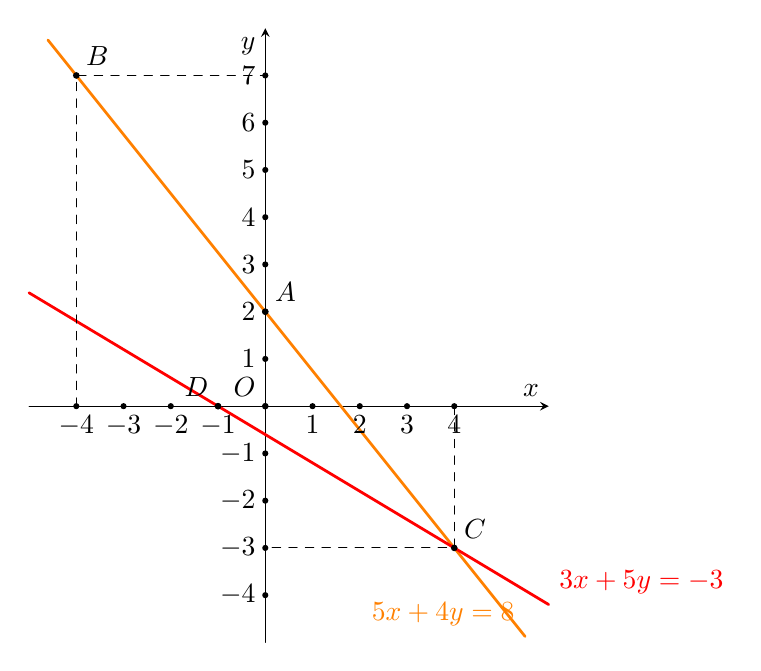
\begin{tikzpicture}[>=stealth,line join=round, line cap=round, scale=0.6]
	\draw[->] (-5,0)--(6,0) node[above left]{$x$};
	\draw[->] (0,-5)--(0,8) node[below left]{$y$};
	\draw[samples=200,smooth,orange,line width=1] plot[domain=-4.6:5.5] 
	(\x,{2-(5/4)*\x}) node[above left]{$5x+4y=8$};
	\draw[samples=200,smooth,red,line width=1] plot[domain=-5:6] 
	(\x,{-3/5-(3/5)*\x}) node[above right]{$3x+5y=-3$};
	\foreach \x in {-4,-3,-2,-1,1,2,3,4} \draw[fill] (\x,0) circle (1.5pt) 
	node[below]{$\x$};
	\foreach \y in {-4,-3,-2,-1,1,2,3,4,5,6,7} \draw[fill] (0,\y) circle (1.5pt) 
	node[left]{$\y$};
	\draw[dashed] (-4,0)--(-4,7)--(0,7);
	\draw[dashed] (4,0)--(4,-3)--(0,-3);
	\fill (0,0) circle (2pt) node[above left]{$O$};
	\fill (0,2) circle (2pt) node[above right]{$A$};
	\fill (-4,7) circle (2pt) node[above right]{$B$};
	\fill (4,-3) circle (2pt) node[above right]{$C$};
	\fill (-1,0) circle (2pt) node[above left]{$D$};
	\end{tikzpicture}
	\end{center}
	\end{enumerate}
	}
\end{bt}
\begin{bt}%[9D3B1]
	Tìm $m$ biết $( - 1 ; - 1)$ là một nghiệm của phương trình 
	$(m - 1) x - (2m - 1) y = - 1 - m.$
	\dapso{$m=-\dfrac{1}{2}$.}
	\loigiai{$m=-\dfrac{1}{2}$}
\end{bt}
\begin{bt}%[9D3K1]
	Cho phương trình $3x + 2y = 6$ \hfill $(1)$
	\begin{enumerate}
	\item Hãy biểu diễn tập nghiệm của phương trình $(1)$ trên mặt phẳng tọa độ (gọi là $(d)$).
	\item Tính diện tích tam giác tạo bởi $(d)$ với trục $Ox$ và $Oy$.
	\end{enumerate}
	\loigiai
	{
	\immini
	{
	\begin{enumerate}
	\item Tập nghiệm của phương trình $3x + 2y = 6$ được biểu diễn như hình bên.
	\item Diện tích tam giác tạo bởi $(d)$ với trục $Ox$ và $Oy$
	\[\mathrm{S}=\dfrac{1}{2}\cdot\mathrm{OA}\cdot\mathrm{OB}=\dfrac{1}{2}\cdot 3\cdot 2 = 3~\text{(đvdt)}.\]
	\end{enumerate}
	}
	{
	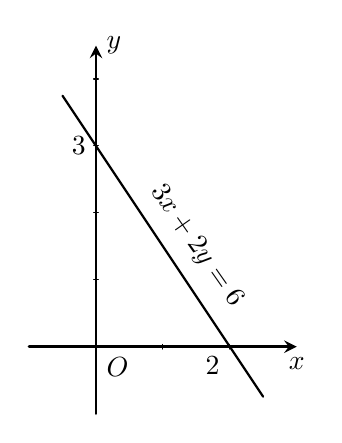
\begin{tikzpicture}[line join = round, line cap = round,>=stealth,thick,scale=0.85]
	\tkzDefPoints{2/0/B,0/3/A}
	\draw[samples=200,domain=-0.5:2.5,smooth] plot (\x, {-3/2*\x + 3}) node[rotate=-55] at (1.5,1.5) {$3x+2y=6$};
	\draw[->,line width = 1pt] (-1,0)--(0,0) node[below right]{$O$}--(3,0) node[below]{$x$};
	\draw[->,line width = 1pt] (0,-1)--(0,4.5) node[right]{$y$};
	\foreach \x in {1,2} \draw[thin] (\x,1pt)--(\x,-1pt);
	\foreach \y in {1,2,3,4} \draw[thin] (1pt,\y)--(-1pt,\y);
	\node at (0,3) [left]{$3$};
	\node at (2,0) [below left]{$2$};
	\tkzDrawPoints[fill=black,,size=2](A,B)
	\tkzLabelPoints[right](A)
	\tkzLabelPoints[above right](B)
	\end{tikzpicture}	
	}
	}
\end{bt}
%%%%%%%%%%%%%%%
%%=====Bài 3
\begin{bt}
Viết nghiệm và biểu diễn hình học tất cả các nghiệm của mỗi phương trình bậc nhất hai ẩn sau:
\begin{enumEX}{3}
	\item $2x-y=3$;
	\item $0x+2y=-4$;
	\item $3x+0y=5$.
\end{enumEX}
\loigiai{
	\begin{enumerate}
	\item 
	\immini{	Xét phương trình $2x-y=3$. \quad $(1)$\\
	Ta viết $(1)$ dưới dạng $y=2x -3$. Mỗi cặp số $(x;2x -3)$ với $x \in \mathbb{R}$ tùy ý, là một nghiệm của $(1)$. Khi đó ta nói phương trình $(1)$ có nghiệm (tổng quát) là:
	\begin{center}
	$(x;2x -3)$ với $x \in \mathbb{R}$ tùy ý.
	\end{center}}{
	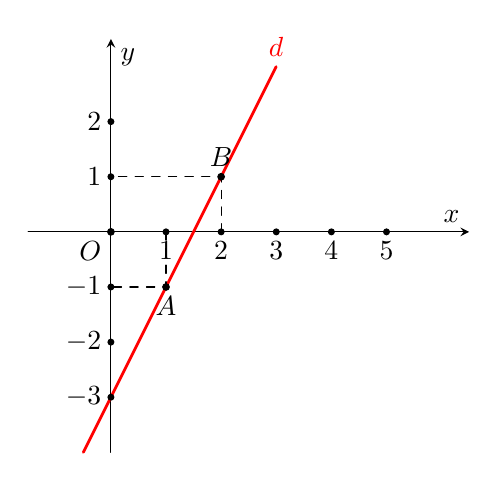
\begin{tikzpicture}[>=stealth,line join=round, line cap=round, scale=0.7]
	\draw[->] (-1.5,0)--(6.5,0) node[above left]{$x$};
	\draw[->] (0,-4)--(0,3.5) node[below right]{$y$};
	\draw[samples=200,smooth,red,line width=1] plot[domain=-0.5:3] 
	(\x,{(2*\x)-3}) node[above]{$d$};
	\foreach \x in {1,2,3,4,5} \draw[fill] (\x,0) circle (1.5pt) 
	node[below]{$\x$};
	\foreach \y in {-3,-2,-1,1,2} \draw[fill] (0,\y) circle (1.5pt) 
	node[left]{$\y$};
	\draw[dashed] (1,0)--(1,-1)--(0,-1);
	\draw[dashed] (2,0)--(2,1)--(0,1);
	\fill (0,0) circle (2pt) node[below left]{$O$};
	\fill (1,-1) circle (2pt) node[below]{$A$};
	\fill (2,1) circle (2pt) node[above]{$B$};
	\end{tikzpicture}
	}
	Mỗi nghiệm này là tọa độ của một điểm thuộc đường thẳng $y=2x -3$. Ta cũng gọi đường thẳng này là đường thẳng $d: 2x-y=3$.\\
	Để vẽ đường thẳng $d$, ta chỉ cần xác định hai điểm tùy ý của nó, chẳng hạn $A(1;-1)$ và $B(2;1)$ rồi vẽ đường thẳng đi qua hai điểm đó.
	\item 
	\immini{Xét phương trình $0x+2y=-4$. \quad $(2)$\\
	Ta viết gọn $(2)$ thành $y=-2$. Phương trình $(2)$ có nghiệm là $(x;-2)$ với $x \in \mathbb{R}$ tùy ý.\\
	Mỗi nghiệm này là tọa độ của một điểm thuộc đường thẳng song song với trục hoành và cắt trục tung tại điểm $(0;-2)$. Ta gọi đó là đường thẳng $y=-2$ (H1.4b).}{
	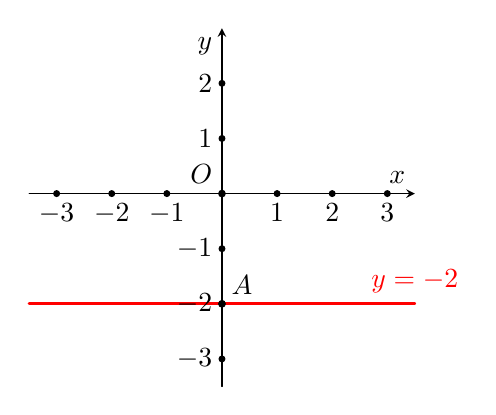
\begin{tikzpicture}[>=stealth,line join=round, line cap=round, scale=0.7]
	\draw[->] (-3.5,0)--(3.5,0) node[above left]{$x$};
	\draw[->] (0,-3.5)--(0,3) node[below left]{$y$};
	\draw[samples=200,smooth,red,line width=1] plot[domain=-3.5:3.5] 
	(\x,{-2}) node[above]{$y=-2$};
	\foreach \x in {-3,-2,-1,1,2,3} \draw[fill] (\x,0) circle (1.5pt) 
	node[below]{$\x$};
	\foreach \y in {-3,-2,-1,1,2} \draw[fill] (0,\y) circle (1.5pt) 
	node[left]{$\y$};
	\fill (0,0) circle (2pt) node[above left]{$O$};
	\fill (0,-2) circle (2pt) node[above right]{$A$};
	\end{tikzpicture}
	}
	\item 
	\immini{Xét phương trình $3x+0y=5$. \quad $(3)$\\
	Ta viết gọn $(3)$ thành $x=\dfrac{5}{3}$. Phương trình $(3)$ có nghiệm là $\left(\dfrac{5}{3};y\right)$ với $x \in \mathbb{R}$ tùy ý.\\
	Mỗi nghiệm này là tọa độ của một điểm thuộc đường thẳng song song với trục tung và cắt trục hoành tại điểm $\left(\dfrac{5}{3};0\right)$. Ta gọi đó là đường thẳng $x=\dfrac{5}{3}$.}{
	\begin{tikzpicture}[>=stealth,line join=round, line cap=round, scale=0.7]
	\draw[->] (-3.5,0)--(3.5,0) node[above left]{$x$};
	\draw[->] (0,-3.5)--(0,3) node[below left]{$y$};
	\draw[-] (1.67,-3.5)--(1.67,3) node[below right]{$x=\tfrac{5}{3}$};
	\foreach \x in {-3,-2,-1,1,2,3} \draw[fill] (\x,0) circle (1.5pt) 
	node[below]{$\x$};
	\foreach \y in {-3,-2,-1,1,2} \draw[fill] (0,\y) circle (1.5pt) 
	node[left]{$\y$};
	\fill (0,0) circle (2pt) node[above left]{$O$};
	%	\fill (0,-2) circle (2pt) node[above right]{$A$};
	\end{tikzpicture}
	}
\end{enumerate}
}
\end{bt}
\begin{bt}%[9D3K1]
	Cho phương trình $3x + 5y = 501$. Hỏi phương trình có bao nhiêu nghiệm nguyên dương?
	\dapso{Phương trình có $33$ nghiệm nguyên dương.}
	\loigiai{Phương trình có $33$ nghiệm nguyên dương.}
\end{bt}
%%%%%%
\begin{bt}
	Hãy biểu diễn tất cả các nghiệm của mỗi phương trình sau trên mặt phẳng tọa độ $Oxy$.
	\begin{listEX}[4]
	\item $2 x+y=3$;
	\item $0 x-y=3$;
	\item $-3 x+0 y=2$;
	\item $-2 x+y=0$.
	\end{listEX}
	\loigiai{
	\immini{
	\begin{enumerate}
	\item Viết lại phương trình thành $y=-2x+3$. Từ đó, tất cả các nghiệm của phương trình đã cho được biểu diễn bởi đường thẳng $d:y=-2x+3$.
	\end{enumerate}
	}{
	\begin{tikzpicture}[>=stealth,scale=1]
	\def\a{-2}
	\def\b{3}
	\draw[->] (-2,0) -- (3,0) node[below] {\scriptsize $x$};
	\draw[->] (0,-1) -- (0,4) node[left] {\scriptsize $y$};
	\fill (0,0) circle (1pt) node[below right]{\scriptsize $O$};
	\foreach \x in {-1,1,2}{\draw (\x,-0.1)--++(90:0.2)node[above]{$\x$};}
	\foreach \y in {1,2,3}{\draw (0.1,\y)--++(180:0.2)node[left]{$\y$};}
	\clip (-2,-1)rectangle(3,4);
	\draw[thick,samples=150,smooth,domain=-2:3,red] plot(\x,{\a*\x+(\b)})node[above left]{$d$};
	\fill (1.5,0) circle (1pt)node[below]{\scriptsize $\tfrac{3}{2}$};
	\end{tikzpicture}
	}
	\immini{
	\begin{enumerate}
	\item[b)] Viết lại phương trình thành $y=-3$. Từ đó, tất cả các nghiệm của phương trình đã cho được biểu diễn bởi đường thẳng $d$ vuông góc với $Oy$ tại điểm $M(0;-3)$.
	\end{enumerate}
	}{
	\begin{tikzpicture}[>=stealth,scale=1]
	\def\a{0}
	\def\b{-3}
	\draw[->] (-2,0) -- (2,0) node[below] {\scriptsize $x$};
	\draw[->] (0,-4) -- (0,1) node[left] {\scriptsize $y$};
	\fill (0,0) circle (1pt) node[below right]{\scriptsize $O$};
	\foreach \x in {-1,1}{\draw (\x,-0.1)--++(90:0.2)node[above]{$\x$};}
	\foreach \y in {-1}{\draw (-0.1,\y)--++(0:0.2)node[right]{$\y$};}
	\clip (-2,-4)rectangle(2,1);
	\draw[thick,samples=150,smooth,domain=-2:2,red] plot(\x,{\a*\x+(\b)})node[above left]{$d$};
	\fill (0,-3) circle (1pt)node[below left]{$-3$};
	\node[below right] at (0,-3){$M$};
	\end{tikzpicture}
	}
	\immini{
	\begin{enumerate}
	\item[c)] Viết lại phương trình thành $x=\dfrac{-2}{3}$. Từ đó, tất cả các nghiệm của phương trình đã cho được biểu diễn bởi đường thẳng $d$ vuông góc với $Ox$ tại điểm $N\left(\dfrac{-2}{3};0\right)$.
	\end{enumerate}
	}{
	\begin{tikzpicture}[>=stealth,scale=1]
	\draw[->] (-3,0) -- (1,0) node[below] {\scriptsize $x$};
	\draw[->] (0,-1) -- (0,3) node[left] {\scriptsize $y$};
	\fill (0,0) circle (1pt) node[below right]{\scriptsize $O$};
	\foreach \x in {-2,-1}{\draw (\x,0.1)--++(-90:0.2)node[below]{$\x$};}
	\foreach \y in {1,2}{\draw (-0.1,\y)--++(0:0.2)node[right]{$\y$};}
	\draw[thick,samples=150,smooth,red] (-2/3,-1)--(-2/3,3);
	\fill (-2/3,0) circle (1pt)node[above right]{\scriptsize $\tfrac{-2}{3}$};
	\node[above left] at (-2/3,0){\scriptsize $N$};
	\end{tikzpicture}
	}
	\immini{
	\begin{enumerate}
	\item[d)] Viết lại phương trình thành $y=2x$. Từ đó, tất cả các nghiệm của phương trình đã cho được biểu diễn bởi đường thẳng $d:y=2x$.
	\end{enumerate}
	}{
	\begin{tikzpicture}[>=stealth,scale=1]
	\def\a{2}
	\def\b{0}
	\draw[->] (-2,0) -- (3,0) node[below] {\scriptsize $x$};
	\draw[->] (0,-1) -- (0,4) node[left] {\scriptsize $y$};
	\fill (0,0) circle (1pt) node[below right]{\scriptsize $O$};
	\foreach \x in {-1,1,2}{\draw (\x,0.1)--++(-90:0.2)node[below]{$\x$};}
	\foreach \y in {1,2,3}{\draw (0.1,\y)--++(180:0.2)node[left]{$\y$};}
	\draw[dashed] (1,0)|-(0,2);
	\clip (-2,-1)rectangle(3,4);
	\draw[thick,samples=150,smooth,domain=-2:3,red] plot(\x,{\a*\x+(\b)});
	\fill (1,2) circle (1pt)
	(0,0) circle (1pt);
	\node[above left] at (1.5,3){$d$};
	\end{tikzpicture}
	}
	}
\end{bt}
\begin{bt}%[9D3K1]
	Tìm nghiệm nguyên của các phương trình sau:
	\begin{listEX}[5]
	\item $2x+y=4$
	\item $x-7y=9$
	\item $x-2y=3$
	\item $3x-2y=4$
	\item $3x+y=8$
	\end{listEX}
	\loigiai{
	\begin{enumerate}
	\item Biến đổi phương trình về dạng $y=-2x+4$.\\
	Nhận xét rằng, với mọi $x\in \mathbb{Z}$, ta luôn có $y=-2x+4\in \mathbb{Z}$.\\
	Vậy phương trình có vô số nghiệm nguyên thỏa mãn $(x;-2x+4)$ với $x\in \mathbb{Z}$.
	\item Biến đổi phương trình về dạng $x=7y+9$.\\
	Nhận xét rằng với mọi $y\in \mathbb{Z}$ ta luôn có $x=7y+9\in \mathbb{Z}$.\\
	Vậy phương trình có vô số nghiệm nguyên thỏa mãn $(7y+9;y)$ với $y\in \mathbb{Z}$.
	\item Biến đổi phương trình về dạng $x=2y+3$.\\
	Nhận xét rằng, với mọi $y\in \mathbb{Z}$, ta luôn có $x=2y+3\in \mathbb{Z}$.\\
	Vậy phương trình có vô số nghiệm nguyên thỏa mãn $(2y+3;y)$ với $y\in \mathbb{Z}$.
	\item Biến đổi phương trình về dạng $2y=3x-4\Leftrightarrow y=-2+x+\dfrac{1}{2}x\quad (1)$.\\
	Đặt $k=\dfrac{1}{2}x,k\in \mathbb{Z}\Leftrightarrow x=2k,k\in \mathbb{Z}$.\\
	Thay $x=2k$ vào $(1)$ ta được $y=-2+2k+k=-2+3k\in \mathbb{Z},k\in \mathbb{Z}$.\\
	Vậy phương trình có vô số nghiệm nguyên thỏa mãn $(2k;-2+3k),$ với $k\in \mathbb{Z}$.
	\item Biến đổi phương trình về dạng $y=-3x+8$.\\
	Nhận xét rằng, với mọi $x\in \mathbb{Z}$, ta luôn có $y=-3x+8\in \mathbb{Z}$.\\
	Vậy phương trình đã cho có vô số nghiệm nguyên thỏa mãn $(x;-3x+8)$, với $x\in \mathbb{Z}$.
	\end{enumerate}
	}
\end{bt}
\begin{bt}%[9D3G1]
	Chứng minh rằng khi $m$ thay đổi, các đường thẳng sau luôn đi qua một điểm cố định.
	\begin{listEX}[2]
	\item $m(x-5)-2y=6$;
	\item $mx-2y=6$.
	\end{listEX}
	\loigiai{
	\begin{enumerate}
	\item Giả sử $M(x_0;u_0)$ là điểm cố định mà đường thẳng luôn đi qua. Khi đó ta có\\
	$m(x_0-5)-2y_0=6\,\forall m\Leftrightarrow\heva{&x_0-5=0\\&-2y_0-6=0}\Leftrightarrow\heva{&x_0=5\\&y_0=-3}$.\\
	Vậy $M(5;-3)$ là điểm cố định mà đường thẳng luôn đi qua khi $m$ thay đổi.
	\item Giả sử $M(x_0;y_0)$ là điểm cố định mà đường thẳng luôn đi qua. Khi đó ta có\\
	$mx_0-2y_0=6\Leftrightarrow\heva{&x_0=0\\&-2y_0-6=0}\Leftrightarrow\heva{&x_0=0\\&y_0=-3.}$\\
	Vậy $M(0;-3)$ là điểm cố định mà đường thẳng luôn đi qua khi $m $ thay đổi.
	\end{enumerate}
	}
\end{bt}
\begin{bt}
	Cho hệ phương trình $\heva{&4 x-y=2 \\&x+3 y=7}$. Cặp số nào dưới đây là nghiệm của hệ phương trình đã cho?
	\begin{listEX}[3]
	\item $(2 ; 2)$; 
	\item $(1 ; 2)$;
	\item $(-1 ;-2)$.
	\end{listEX}
	\loigiai{
	\begin{listEX}
	\item Cặp số $(2 ;2)$ không phải là nghiệm của hệ phương trình vì $\heva{&4\cdot 2-2=6\ne 2 \\ &2+3\cdot2=8\ne 7.}$
	\item Cặp số $(1 ;2)$ là nghiệm của hệ phương trình vì $\heva{&4\cdot 1-2=2 \\ &1+3\cdot2=7.}$
	\item Cặp số $(-1 ;-2)$ không phải là nghiệm của hệ phương trình vì $\heva{&4\cdot (-1)-2=-6 \ne 2\\ &-1+3\cdot(-2)=-7\ne7 .}$
	\end{listEX}	
	}
\end{bt}
\begin{bt}
	\begin{enumerate}
	\item Hệ phương trình $\heva{&2x=-6 \\&5x+4y=1}$ có là một hệ hai phương trình bậc nhất hai ẩn không, vì sao?
	\item Cặp số $(-3;4)$ có là một nghiệm của hệ phương trình đó hay không, vì sao?
	\end{enumerate}
	\loigiai{
	\begin{enumerate}
	\item Các phương trình $2x+0y=-6$ và $5x+4y=1$ thỏa mãn điều kiện $a \ne 0$ hoặc $b \ne 0$ nên là phương trình bậc nhất hai ẩn. Do đó hệ phương trình $\heva{&2x=-6 \\&5x+4y=1}$ là hệ hai phương trình bậc nhất hai ẩn.
	\item 	Ta thấy khi $x=-3$ và $y=4$ thì:\\
	$2x=2\cdot (-3)=-6$ nên $(-3;4)$ là nghiệm của phương trình thứ nhất;\\
	$5x+4y=5 \cdot (-3) +4 \cdot 4=1$ nên $(-3;4)$ là nghiệm của phương trình thứ hai.\\
	Vậy $(-3;4)$ là nghiệm chung của hai phương trình, nghĩa là $(-3;4)$ là một nghiệm của hệ phương trình đã cho.\\
	\end{enumerate}
	}
\end{bt}
\begin{bt}
	Cho hai đường thẳng $y=-\dfrac{1}{2}x+2$ và $y=-2x-1$.
	\begin{listEX}
	\item Vẽ hai đường thẳng đó trên cùng một hệ trục tọa độ.
	\item Xác định tọa độ giao điểm $A$ của hai đường thẳng trên.
	\item Tọa độ của điểm $A$ có là nghiệm của hệ phương trình $\heva{&x+2 y=4 \\ &2 x+y=-1}$ không? Tại sao?
	\end{listEX}
	\loigiai{
	\begin{listEX}
	\item Vẽ hai đường thẳng $y=-\dfrac{1}{2}x+2$ và $y=-2x-1$ trên cùng một hệ trục tọa độ.\\
	\immini{
	Bảng giá trị của hàm số $y = -2x - 1$.
	\begin{center}
	\begin{tabular}{|c|c|c|}
	\hline
	$x$	& $0$ & $-1$ \\
	\hline
	$y = -2x - 1$	& $-1$ & $1$ \\
	\hline
	\end{tabular} 
	\end{center}
	Bảng giá trị của hàm số $y = -\dfrac{1}{2}x +2$.
	\begin{center}
	\begin{tabular}{|c|c|c|}
	\hline \rule[-16pt]{0pt}{35pt}
	$x$	& $0$ & $2$ \\
	\hline \rule[-16pt]{0pt}{35pt}
	$y = -\dfrac{1}{2}x + 2$	& $2$ & $1$ \\
	\hline
	\end{tabular}
	\end{center}
	Vẽ đồ thị
	}{
	\begin{tikzpicture}[>=stealth,scale=1]
	\def\a{-0.5};\def\b{2};\def\c{-2};\def\d{-1};
	\draw[->] (-4,0) -- (2,0) node[below] {\scriptsize $x$};
	\draw[->] (0,-1) -- (0,5) node[left] {\scriptsize $y$};
	\fill (0,0) circle (1pt) node[below right]{\scriptsize $O$};
	\foreach \x in {-3,-2,-1,1}{\draw (\x,0.1)--++(-90:0.2)node[below]{$\x$};}
	\foreach \y in {1,2,3,4}{\draw (-0.1,\y)--++(0:0.2)node[right]{$\y$};}
	\draw[dashed] (-2,0)|-(0,3);
	\clip (-4,-1)rectangle(2,5);
	\draw[thick,samples=150,smooth,domain=-4:2,red] plot(\x,{\a*\x+(\b)});
	\draw[thick,samples=150,smooth,domain=-4:2,red] plot(\x,{\c*\x+(\d)});
	\fill (1,2) circle (1pt)
	(0,0) circle (1pt);
	\node[rotate=-26.5,below] at (-3,3.5){\scriptsize $y=\tfrac{-1}{2}x+2$};
	\node[rotate=-63.5,above] at (-1.2,1.4){\scriptsize $y=-2x-1$};
	\end{tikzpicture}
	}
	\item Phương trình hoành độ giao điểm của đường thẳng $y=-\dfrac{1}{2}x+2$ và $y=-2x-1$ là \[\dfrac{1}{2}x+2=-2x-1\Leftrightarrow x=-2\Rightarrow y=-2\cdot (-2)-1=3.\]
	Vậy $ (-2;3) $ là tọa độ giao điểm của đường thẳng $y=-\dfrac{1}{2}x+2$ và $y=-2x-1$.
	\item Cặp số $(-2 ;3)$ là nghiệm của hệ phương trình vì $\heva{&-2+2\cdot 3=4\\ &2\cdot(-2)+3=-1.}$
	\end{listEX}
	}
\end{bt}
%---------------
%%=====Bài 3
\begin{bt}
	\immini{
	Nhân dịp tết Trung thu, một doanh nghiệp dự định sản xuất hai loại bánh: bánh nướng và bánh dẻo. Lượng đường cần cho mỗi chiếc bánh nướng, bánh dẻo lần lượt là $60$g và $50$g. Gọi $x$ và $y$ lần lượt là số lượng bánh nướng và bánh dẻo mà doanh nghiệp dự định sản xuất để lượng đường sản xuất bánh là $500$kg. Viết phương trình bậc nhất hai ẩn $x,y$ và chỉ ra ba nghiệm của phương trình đó.
	}{
	
\includegraphics[scale=0.7]{images/9C1-2-1.jpg}
	}
	\loigiai{
	Ta có $500$kg = $500~000$g.\\
	Lượng đường để doanh nghiệp sản xuất $x$ cái bánh nướng là $60x$ (g).\\
	Lượng đường để doanh nghiệp sản xuất $y$ cái bánh dẻo là $50y$ (g).\\
	Lượng đường để doanh nghiệp sản xuất cả hai loại bánh là $500~000$ (g).\\ 
	Do đó ta có phương trình
	$$60x+50y=500~000 \text{ hay } 6x+5y=50~000. \quad (1)$$
	\begin{itemize}
	\item Thay $x=5000, y=4000$ vào phương trình $(1)$ ta có $6\cdot 5000+5\cdot 4000=50~000$.\\ 
	$\Rightarrow \left(5000;4000\right)$ là một nghiệm của phương trình $(1)$.
	\item Thay $x=4000, y=5200$ vào phương trình $(1)$ ta có $6\cdot 4000+5\cdot 5200=50~000$.\\ 
	$\Rightarrow \left(4000;5200\right)$ là một nghiệm của phương trình $(1)$.
	\item Thay $x=2500, y=7000$ vào phương trình $(1)$ ta có $6\cdot 2500+5\cdot 7000=50~000$.\\ 
	$\Rightarrow \left(2500;7000\right)$ là một nghiệm của phương trình $(1)$.
	\end{itemize}
	}
\end{bt}
%%=====Bài 4
\begin{bt}
	Năm bạn Châu, Hà, Khang, Minh, Phong cùng đi mua sticker để trang trí vở. Có hai loại sticker: loại I giá $2$ nghìn đồng/chiếc và loại II giá $3$ nghìn đồng/chiếc. Mỗi bạn mua $1$ chiếc và tổng số tiền năm bạn phải trả là $12$ nghìn đồng. Gọi $x$ và $y$ lần lượt là số sticker loại I và loại II mà năm bạn đã mua.
	\begin{enumerate}
	\item Viết hệ phương trình bậc nhất hai ẩn $x,y$.
	\item Cặp số $\left(3;2\right)$ có phải là nghiệm của hệ phương trình ở câu a hay không? Vì sao?
	\end{enumerate}
	\loigiai{
	\begin{enumerate}
	\item Gọi $x$ và $y$ lần lượt là số sticker loại I và loại II mà năm bạn đã mua.\\
	Do đó ta có phương trình $x+y=5 \quad (1)$.\\
	Số tiền trả cho sticker loại I là $2x$ nghìn đồng.\\
	Số tiền trả cho sticker loại II là $3y$ nghìn đồng.\\
	Do tổng số tiền năm bạn phải trả là $12$ nghìn đồng nên ta có phương trình
	$$2x+3y=12. \quad (2)$$
	Từ $(1)$ và $(2)$ ta có hệ phương trình bậc nhất hai ẩn
	$$\heva{& x+y=5\\ &2x+3y=12.}$$
	\item Thay giá trị $x=3,y=2$ vào hai phương trình trong hệ, ta có
	\begin{itemize}
	\item $3+2=5$.
	\item $2\cdot 3+3\cdot 2=12$.
	\end{itemize}
	Suy ra cặp số $\left(3;2\right)$ là nghiệm của cả hai phương trình trong hệ.\\
	Do đó cặp số $\left(3;2\right)$ là nghiệm của hệ phương trình trên.
	\end{enumerate}
	}
\end{bt}
%%=====Bài 5
\begin{bt}
	Để chuẩn bị cho buổi liên hoan của gia đình, bác Ngọc mua hai loại thực phẩm là thịt lợn và cá chép. Giá tiền thịt lợn là $130$ nghìn đồng/kg, giá tiền cá chép là $50$ nghìn đồng/kg. Bác Ngọc đã chi $295$ nghìn đồng để mua $3{,}5$ kg hai loại thực phẩm trên. Gọi $x$ và $y$ lần lượt là số kilôgam thịt lợn và cá chép mà bác Ngọc đã mua.
	\begin{enumerate}
	\item Viết hệ phương trình bậc nhất hai ẩn $x,y$.
	\item Cặp số $\left(1{,}5;2\right)$ có phải là nghiệm của hệ phương trình ở câu a hay không? Vì sao?
	\end{enumerate}
	\loigiai{
	\begin{enumerate}
	\item Gọi $x$ và $y$ lần lượt là số kilôgam thịt lợn và cá chép mà bác Ngọc đã mua.\\
	Do bác Ngọc mua $3{,}5$ kg cả hai loại thịt lợn và cá chép nên ta có
	$$x+y=3{,}5. \quad (1)$$
	Số tiền để mua $x$ kg thịt lợn là $130x$ nghìn đồng.\\
	Số tiền để mua $y$ kg cá chép là $50y$ nghìn đồng.\\
	Bác Ngọc đã chi $295$ nghìn đồng để mua hai loại thực phẩm trên nên ta có
	$$130x+50y=295 \text{ hay } 26x+ 10y=59. \quad (2)$$
	Từ $(1)$ và $(2)$ ta có hệ phương trình
	$$\heva{& x+y=3{,}5\\ & 26x+ 10y=59.}$$
	\item Thay giá trị $x=1{,}5,y=2$ vào hai phương trình trong hệ, ta có
	\begin{itemize}
	\item $1{,}5+2=3{,}5$.
	\item $26\cdot 1{,}5+10\cdot 2=59$.
	\end{itemize}
	Suy ra cặp số $\left(1{,}5;2\right)$ là nghiệm của cả hai phương trình trong hệ.\\
	Do đó cặp số $\left(1{,}5;2\right)$ là nghiệm của hệ phương trình trên.
	\end{enumerate}
	}
\end{bt}
%%=====Bài 6
\begin{bt}
	Người ta cần sơn hai loại sản phẩm A, B bằng hai loại sơn: sơn xanh và sơn vàng. Lượng sơn để sơn mỗi loại sản phẩm được cho ở bảng (đơn vị: kg/$1$ sản phẩm).
	\begin{center}
	\begin{tabular}{|c|c|c|}
	\hline 
	\diagbox{Loại sản phẩm}{Loại sơn} & Sơn xanh & Sơn vàng \\
	\hline 
	Sản phẩm loại A & $0{,}6$ & $0{,}3$ \\
	\hline 
	Sản phẩm loại B & $0{,}5$ & $0{,}4$ \\
	\hline 
	\end{tabular}
	\end{center}
	Người ta dự định sử dụng $85$ kg sơn xanh và $50$ kg sơn vàng để sơn tất cả sản phẩm của hai loại đó. Gọi $x,y$ lần lượt là số sản phẩm loại A và số sản phẩm loại B được sơn.
	\begin{enumerate}
	\item Viết hệ phương trình bậc nhất hai ẩn $x,y$.
	\item Cặp số $\left(100;50\right)$ có phải là nghiệm của hệ phương trình ở câu a hay không? Vì sao?
	\end{enumerate}
	\loigiai{
	\begin{enumerate}
	\item Gọi $x,y$ lần lượt là số sản phẩm loại A và số sản phẩm loại B được sơn.\\
	Sơn $x$ sản phẩm loại A cần: $0{,}6x$ kg sơn màu xanh và $0{,}3x$ kg sơn màu vàng.\\
	Sơn $y$ sản phẩm loại B cần: $0{,}5y$ kg sơn màu xanh và $0{,}4y$ kg sơn màu vàng.\\
	Cần sử dụng $85$ kg sơn xanh để sơn tất cả sản phẩm của hai loại nên ta có
	$$0{,}6x+0{,}5y=85 \text{ hay } 6x+5y=850. \quad (1)$$
	Cần sử dụng $50$ kg sơn vàng để sơn tất cả sản phẩm của hai loại nên ta có
	$$0{,}3x+0{,}4y=50 \text{ hay } 3x+4y=500. \quad (2)$$
	Từ $(1)$ và $(2)$ ta có hệ phương trình
	$$\heva{& 6x+5y=850\\ & 3x+4y=500.}$$
	\item Thay giá trị $x=100,y=50$ vào hai phương trình trong hệ, ta có
	\begin{itemize}
	\item $6\cdot 100+5\cdot 50=850$.
	\item $3\cdot 100+4\cdot 50=500$.
	\end{itemize}
	Suy ra cặp số $\left(100;50\right)$ là nghiệm của cả hai phương trình trong hệ.\\
	Do đó cặp số $\left(100;50\right)$ là nghiệm của hệ phương trình trên.
	\end{enumerate}
	}
\end{bt}
\begin{bt}
	Không vẽ đồ thị, hãy đoán nhận số nghiệm của các hệ phương trình sau
	\begin{enumEX}{4} 
	\item $\heva{4x+3y&=5\\x+y&=1;}$
	\item $\heva{x-2y&=5\\-2x+4y&=3;}$
	\item $\heva{3x-y&=2\\-6x+2y&=-4;}$
	\item $\heva{\dfrac{2}{3}x+\dfrac{3}{2}y&=5\\2y&=8.}$
	\end{enumEX}
	\loigiai{
	\begin{enumEX}{2} 
	\item $\heva{4x+3y&=5\\x+y&=1.}$\\
	Do $\dfrac{4}{1} \neq \dfrac{3}{1}$ nên hệ có nghiệm duy nhất.
	\item $\heva{x-2y&=5\\-2x+4y&=3.}$\\
	Do $\dfrac{1}{-2}=\dfrac{-2}{4} \neq \dfrac{5}{3}$ nên hệ vô nghiệm.
	\item $\heva{3x-y&=2\\-6x+2y&=-4.}$\\
	Do $\dfrac{3}{-6}=\dfrac{-1}{2}=\dfrac{2}{-4}$ nên hệ có vô số nghiệm.
	\item $\heva{\dfrac{2}{3}x+\dfrac{3}{2}y&=5\\2y&=8.}$\\
	Do $\dfrac{0}{\dfrac{2}{3}}\neq \dfrac{2}{\dfrac{3}{2}}$ nên hệ có nghiệm duy nhất.
	\end{enumEX}
	}
\end{bt}
\begin{bt}%[9D3K2]
	Không vẽ đồ thị, hãy đoán số nghiệm của mỗi phương trình sau
	\begin{enumEX}{4}
	\item $\begin{cases}
	{2x + y = 4}\\
	{3x - y = 2;}
	\end{cases}$
	\item $\begin{cases}
	{2\cdot x + y\cdot 0 = 4}\\
	{3x - y = 5;}
	\end{cases}$
	\item $\begin{cases}
	{x - 2y = 4}\\
	{2x - 4y = 5;}
	\end{cases}$
	\item $\begin{cases}
	{2x + y = 1}\\
	{x + \dfrac{y}{2}=\dfrac{1}{2}.}
	\end{cases}$
	\end{enumEX}
	\loigiai
	{
	\begin{enumerate}
	\item Có một nghiệm duy nhất.
	\item Có một nghiệm duy nhất.
	\item Vô nghiệm.
	\item Vô số nghiệm.
	\end{enumerate}	
	}
\end{bt}
\begin{bt}
	Cho hệ phương trình $\heva{&3x+ay&=5\\
	&2x+y&=b}.$ Tìm $a,b$ để hệ
	\begin{enumEX}{3}
	\item Có nghiệm duy nhất;
	\item Vô nghiệm;
	\item Vô số nghiệm.
	\end{enumEX}
	\loigiai{\begin{enumEX}{1}
	\item Hệ có nghiệm duy nhất $\Leftrightarrow \dfrac{3}{2} \neq \dfrac{a}{1} \Leftrightarrow a \neq \dfrac{3}{2}.$
	\item Hệ vô nghiệm $\Leftrightarrow \dfrac{3}{2} = \dfrac{a}{1} \neq \dfrac{5}{b} \Leftrightarrow \heva{\dfrac{3}{2} &= \dfrac{a}{1} \\ \dfrac{3}{2} &\neq \dfrac{5}{b}} \Leftrightarrow \heva{a &= \dfrac{3}{2}\\ b &\neq \dfrac{10}{3}.}$
	\item Hệ có vô số nghiệm $\Leftrightarrow \dfrac{3}{2} = \dfrac{a}{1} = \dfrac{5}{b} \Leftrightarrow \heva{\dfrac{3}{2} &= \dfrac{a}{1} \\ \dfrac{3}{2} &= \dfrac{5}{b}} \Leftrightarrow \heva{a &= \dfrac{3}{2}\\ b &= \dfrac{10}{3}.}$
	\end{enumEX}}	
\end{bt}
\begin{bt}%[9D3K2]
	Cho hệ phương trình $\begin{cases}
	{x + y = 3}\\
	{2x + y = 4.}
	\end{cases}$
	\begin{enumerate}
	\item Giải hệ phương trình bằng đồ thị.
	\item Nghiệm của hệ có phải là nghiệm của phương trình $3x - 2y = - 1$ hay không?
	\end{enumerate}
	\loigiai
	{
	\begin{enumerate}
	\item Hệ có nghiệm duy nhất $(1;2)$.
	\item Nghiệm của hệ có là nghiệm của phương trình $3x - 2y = - 1$.
	\end{enumerate}	
	}
\end{bt}
\begin{bt}%[9D3K2]
	Xét hệ phương trình $\begin{cases}
	{a x - y = b}\\
	{a^{\prime}x - y = b.}
	\end{cases}$
	\begin{enumerate}
	\item Chứng minh hệ đã cho luôn có nghiệm với mọi $a$, $a'$, $b$.
	\item Hệ đã cho có thể vô số nghiệm được không?
	\end{enumerate}
	\loigiai
	{
	\begin{enumerate}
	\item Hai đồ thị của hai phương trình luôn cắt nhau tại $(0;-b)$ nên hệ đã cho luôn có nghiệm.
	\item Hệ đã cho có thể có vô số nghiệm khi $a=a'$.
	\end{enumerate}	
	}
\end{bt}	